\documentclass[10pt,landscape]{scrartcl}
\usepackage{multicol}
\usepackage{calc}
\usepackage{ifthen}
\usepackage[landscape]{geometry}
\usepackage{amsmath,amsthm,amsfonts,amssymb}
\usepackage{color,graphicx}
\usepackage{hyperref}
\usepackage[font=scriptsize,labelfont=bf]{caption}
\usepackage{wrapfig}
\usepackage{graphicx,calc}
\usepackage{empheq}
\usepackage{xcolor}
\usepackage{siunitx}
%\usepackage{pbox}

\pdfinfo{
  /Title (Leistungelektronik)
  /Creator (TeX)
  /Producer (pdfTeX 1.40.0)
  /Author (Noah Huetter)
  /Subject (Leistungelektronik)
  /Keywords (Leistungelektronik,ETH)}

\definecolor{section}{RGB}{28,82,83}
\definecolor{titletext}{RGB}{0,0,0}
\definecolor{formula}{RGB}{249,220,155}

\setkomafont{section}{\mysection}
\newcommand{\mysection}[1]{%
    \Large\bf%
    \setlength{\fboxsep}{0cm}%already boxed
    \fcolorbox{black}{gray!40}{%
        \begin{minipage}{\linewidth}%
            \vspace*{2pt}%Space before
            #1
            \vspace*{2pt}%Space after
        \end{minipage}%
    }}

% This sets page margins to .5 inch if using letter paper, and to 1cm
% if using A4 paper. (This probably isn't strictly necessary.)
% If using another size paper, use default 1cm margins.
\ifthenelse{\lengthtest { \paperwidth = 11in}}
    { \geometry{top=.5in,left=.5in,right=.5in,bottom=.5in} }
    {\ifthenelse{ \lengthtest{ \paperwidth = 297mm}}
        {\geometry{top=1cm,left=1cm,right=1cm,bottom=1cm} }
        {\geometry{top=1cm,left=1cm,right=1cm,bottom=1cm} }
    }

% Turn on simple page number
\pagestyle{plain}

% Redefine section commands to use less space
\makeatletter
% \renewcommand{\section}{\@startsection{section}{1}{0mm}%
%                                 {-1ex plus -.5ex minus -.2ex}%
%                                 {0.5ex plus .2ex}%x
%                                 {\normalfont\large\bfseries}}
\renewcommand{\subsection}{\@startsection{subsection}{2}{0mm}%
                                {-1explus -.5ex minus -.2ex}%
                                {0.5ex plus .2ex}%
                                {\normalfont\normalsize\bfseries}}
\renewcommand{\subsubsection}{\@startsection{subsubsection}{3}{0mm}%
                                {-1ex plus -.5ex minus -.2ex}%
                                {1ex plus .2ex}%
                                {\normalfont\small\bfseries}}
\makeatother

% bring the old commands back as needed via:
\makeatletter
\DeclareOldFontCommand{\rm}{\normalfont\rmfamily}{\mathrm}
\DeclareOldFontCommand{\sf}{\normalfont\sffamily}{\mathsf}
\DeclareOldFontCommand{\tt}{\normalfont\ttfamily}{\mathtt}
\DeclareOldFontCommand{\bf}{\normalfont\bfseries}{\mathbf}
\DeclareOldFontCommand{\it}{\normalfont\itshape}{\mathit}
\DeclareOldFontCommand{\sl}{\normalfont\slshape}{\@nomath\sl}
\DeclareOldFontCommand{\sc}{\normalfont\scshape}{\@nomath\sc}
\makeatother

% make smaller enumerates
\usepackage{enumitem}
\setlist[enumerate]{itemsep=-1mm,leftmargin=3mm}

% Define BibTeX command
\def\BibTeX{{\rm B\kern-.05em{\sc i\kern-.025em b}\kern-.08em
    T\kern-.1667em\lower.7ex\hbox{E}\kern-.125emX}}

% Don't print section numbers
\setcounter{secnumdepth}{0}


\setlength{\parindent}{0pt}
\setlength{\parskip}{1pt plus 0.5ex}

%My Environments
\newtheorem{example}[section]{Example}
% -----------------------------------------------------------------------
\newcommand{\eqn}[3]
{
  \begin{minipage}[#1]{#2}
    \[ #3 \]
  \end{minipage}
}
\newcommand{\feqn}[3]
{
\fbox{
  \begin{minipage}[#1]{#2}
    \[ #3 \]
  \end{minipage}
}
}

% equation box        
\newcommand{\eqbox}[1]{\fcolorbox{black}{formula}{\hspace{0.5em}$\displaystyle#1$\hspace{0.5em}}}

\newcommand{\Pabl}[2] {\frac{\partial#1}{\partial#2}}
\newcommand{\MATR}[1]{ \displaystyle \left( \begin{matrix} #1 \end{matrix} \right)}
\newcommand{\MATRABS}[1]{ \displaystyle \left| \begin{matrix} #1 \end{matrix} \right|}
\newcommand{\Int}{\int\limits}
\newcommand\warning{%
 \makebox[1.4em][c]{%
 \makebox[0pt][c]{\raisebox{.1em}{\small!}}%
 \makebox[0pt][c]{\color{red}\Large$\bigtriangleup$}}}%

% \DeclareSIUnit[]\\textup{rms}
% {\text{\ensuremath{m_{\textup{p}}}}}

 
\begin{document}
\raggedright
\footnotesize
\begin{multicols}{2}



% multicol parameters
% These lengths are set only within the two main columns
%\setlength{\columnseprule}{0.25pt}
\setlength{\premulticols}{1pt}
\setlength{\postmulticols}{1pt}
\setlength{\multicolsep}{1pt}
\setlength{\columnsep}{2pt}

\begin{center}
     \Large{\underline{Leistungelektronik}} \\
\end{center}
% -----------------------------------------------------------------------
\IfFileExists{../build/revision.tex}{
  \input{../build/revision.tex}
  Author: Noah Huetter \hfill Date: \compiledate \hspace{1em} Commit: \revision
}{Author: Noah Huetter}


% -----------------------------------------------------------------------
 \vspace{2mm} \hrule
\section{Allgemein}
\subsection{Spule und Kondensator}
\begin{align*}
   i_L(t) &= \frac{1}{L}\int u_L(t)\mathrm{d}t &
   u_L(t) &= L\frac{\mathrm{d}}{\mathrm{d}t}i_L(t) &
   i_C(t) &= C\frac{\mathrm{d}}{\mathrm{d}t}u_C(t) &
   u_C(t) &= \frac{1}{C}\int i_C(t)\mathrm{d}t 
\end{align*}


\eqn{h}{0.15\linewidth}{ Q=C\cdot U }


\subsection{Effektiv- und Mittelwerte}

\begin{tabular}{p{0.2\linewidth} p{0.2\linewidth} p{0.2\linewidth} p{0.2\linewidth} }
  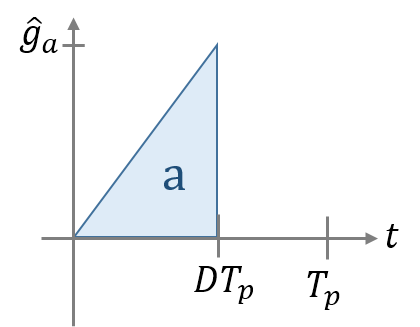
\includegraphics[width=1.0\linewidth]{img/rms/signal_a.png}%
  &
  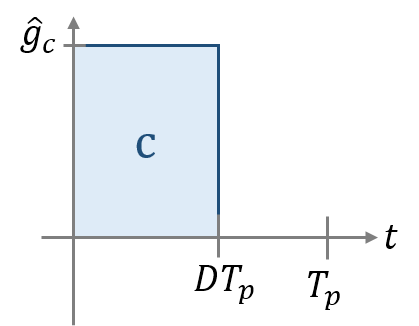
\includegraphics[width=1.0\linewidth]{img/rms/signal_c.png}%
  &
  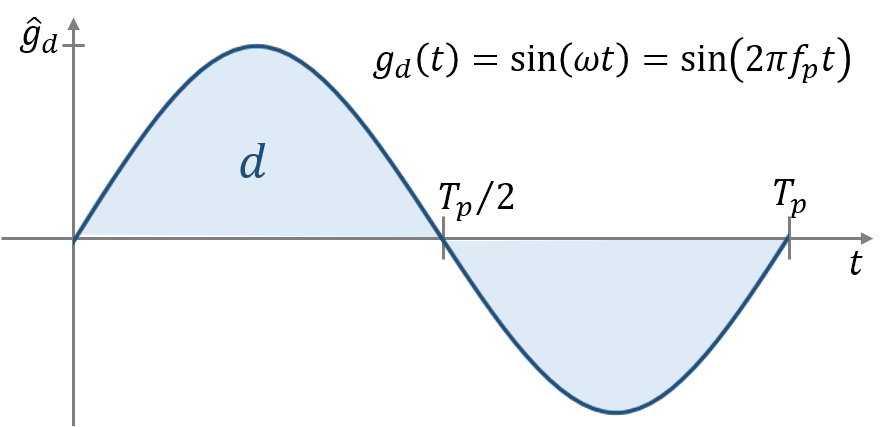
\includegraphics[width=1.0\linewidth]{img/rms/signal_d.png}%
  &
  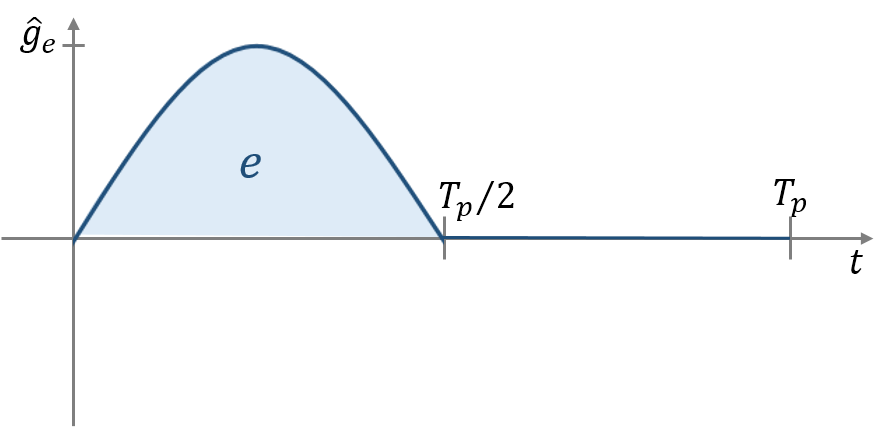
\includegraphics[width=1.0\linewidth]{img/rms/signal_e.png}%
  \\
  {\begin{align*}
    a_{\textup{avg}}   &= \frac{1}{2}\hat{g}_a D \\
    a_{\textup{rms}}^2 &= \frac{1}{3}\hat{g}_a^2 D
  \end{align*}}
  &
  {\begin{align*}
    c_{\textup{avg}}   &= \hat{g}_c D \\
    c_{\textup{rms}}^2 &= \hat{g}_c^2 D
  \end{align*}}
  &
  {\begin{align*}
    d_{\textup{avg}}   &= 0 \\
    d_{\textup{rms}}^2 &= \frac{1}{2}\hat{g}_d^2
  \end{align*}}
  &
  {\begin{align*}
    e_{\textup{avg}}   &= \frac{1}{\pi}\hat{g}_e \\
    e_{\textup{rms}}^2 &= \frac{1}{4}\hat{g}_e^2
  \end{align*}}
\end{tabular}
\begin{center}
\begin{tabular}{p{0.2\linewidth} p{0.2\linewidth} p{0.2\linewidth} }
  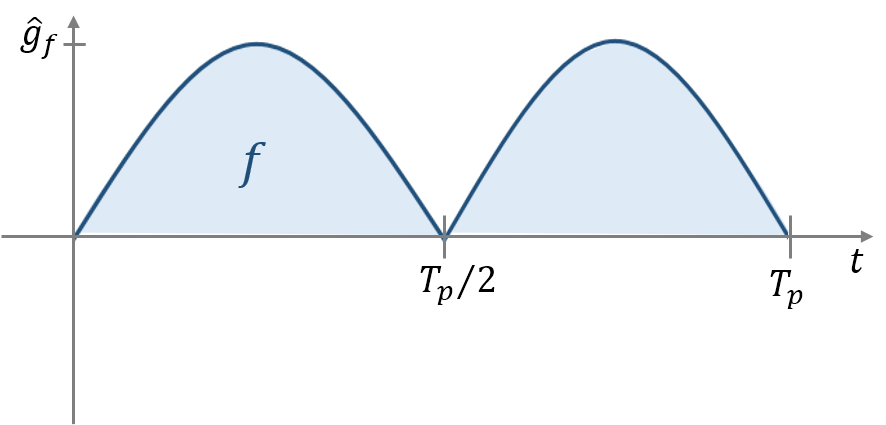
\includegraphics[width=1.0\linewidth]{img/rms/signal_f.png}%
  &
  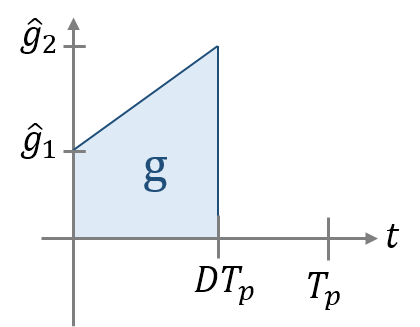
\includegraphics[width=1.0\linewidth]{img/rms/signal_g.png}%
  &
  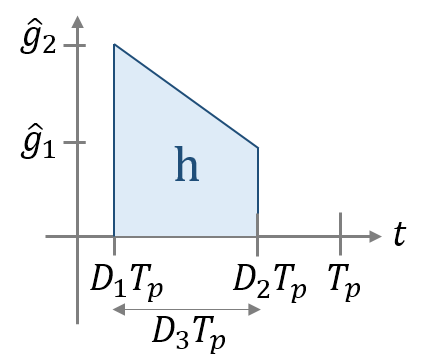
\includegraphics[width=1.0\linewidth]{img/rms/signal_h.png}%
  \\
  {\begin{align*}
    f_{\textup{avg}}   &= \frac{2}{\pi}\hat{g}_f \\
    f_{\textup{rms}}^2 &= \frac{1}{2}\hat{g}_f^2
  \end{align*}}
  &
  {\begin{align*}
    g_{\textup{avg}}   &= \frac{1}{2}(\hat{g}_1+\hat{g}_2) D \\
    g_{\textup{rms}}^2 &= \frac{1}{3}(\hat{g}_1^2 + \hat{g}_1\hat{g}_2+\hat{g}_2^2) D
  \end{align*}}
  &
  {\begin{align*}
    h_{\textup{avg}}   &= \frac{1}{2}(\hat{g}_1+\hat{g}_2) D_3 \\
    h_{\textup{rms}}^2 &= \frac{1}{3}(\hat{g}_1^2 + \hat{g}_1\hat{g}_2+\hat{g}_2^2) D_3
  \end{align*}}
\end{tabular}
\end{center}

% -----------------------------------------------------------------------
\vfill\null
\columnbreak
\section{Tiefsetzsteller}

\begin{center}
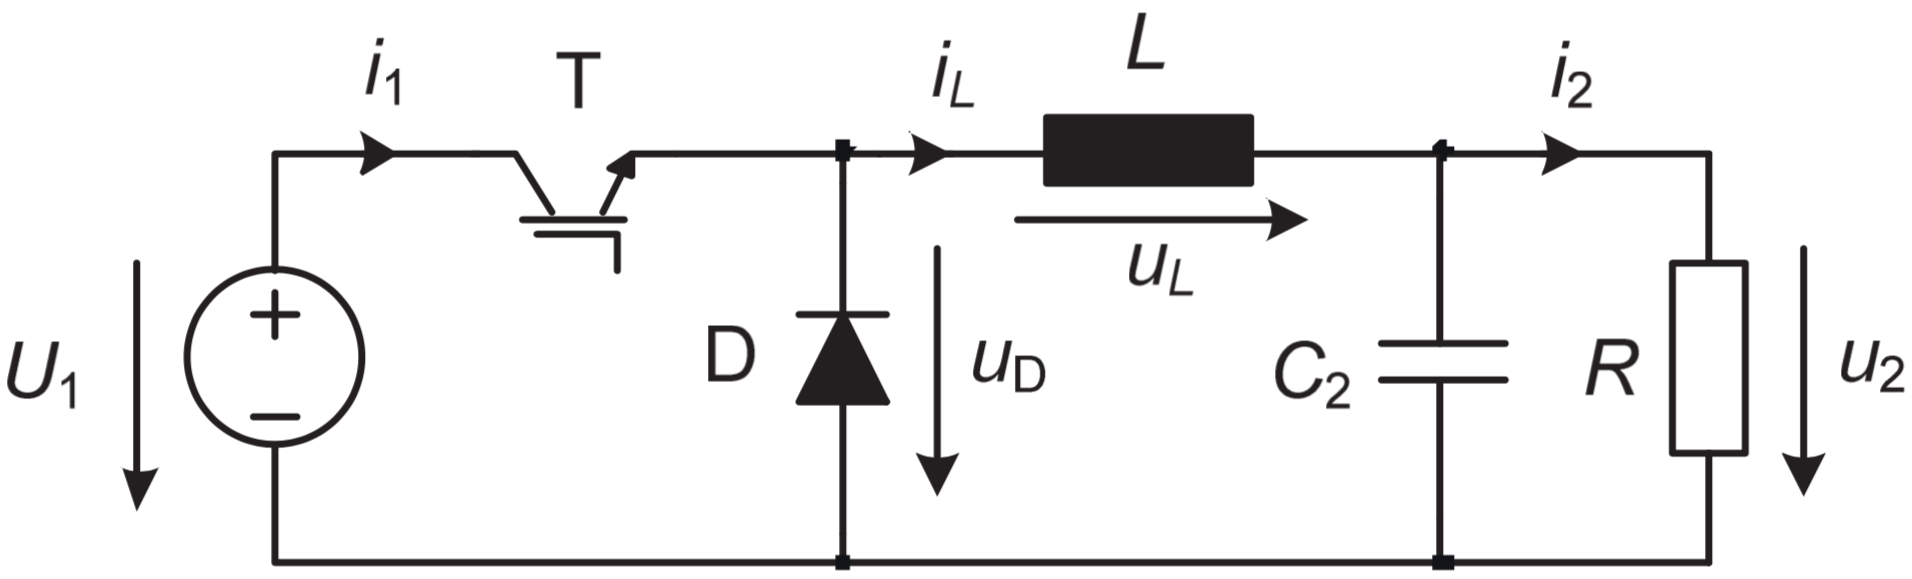
\includegraphics[width=0.8\linewidth]{img/sch_buck.png}%
% \captionof{figure}{Tiefsetzsteller}%
\end{center}

\subsection{Kontinuierlicher Stromfluss}

\begin{tabular}{c c}
  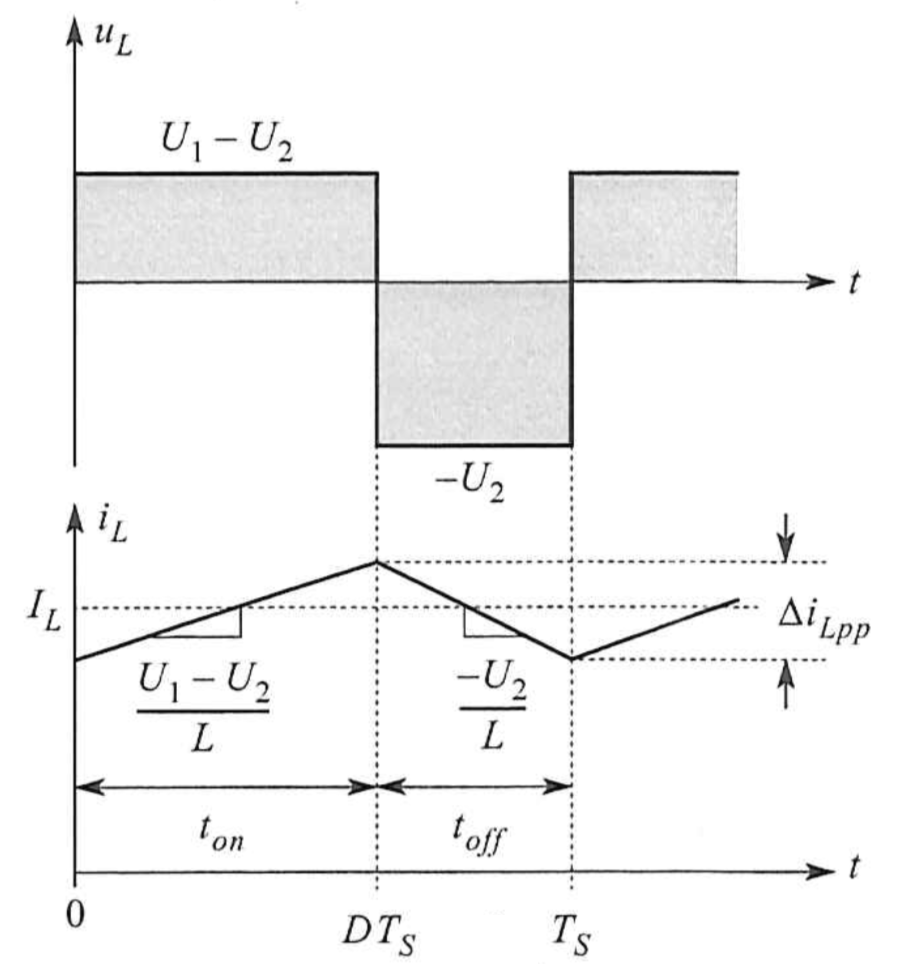
\includegraphics[width=0.4\linewidth]{img/buck/cont.png}%
  &
  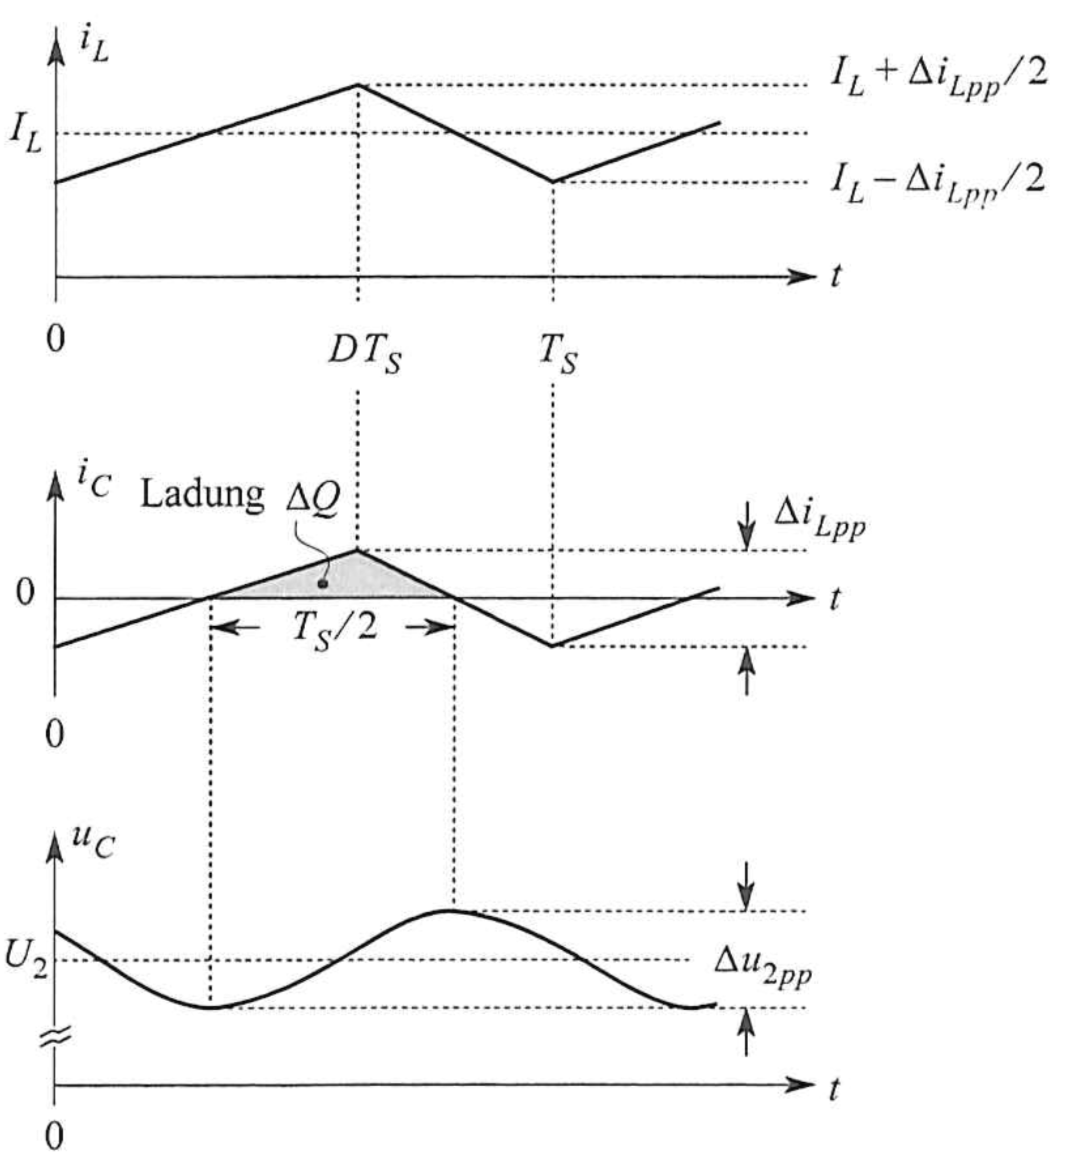
\includegraphics[width=0.4\linewidth]{img/buck/out.png}%
\end{tabular}

\feqn{h}{0.25\linewidth}{ D = \frac{I_1}{I_2} = \frac{U_2}{U_1} }
\eqn{h}{0.25\linewidth}{ \Delta i_{Lpp} = \frac{U_2}{L}(1-D)T_S}
\eqn{h}{0.25\linewidth}{ \Delta u_{2pp}=\Delta U_C = \frac{U_2}{L}(1-D) T_S \frac{T_S}{8 \cdot C}}

\subsection{Diskontinuierlicher Stromfluss}
\begin{tabular}{c c}
  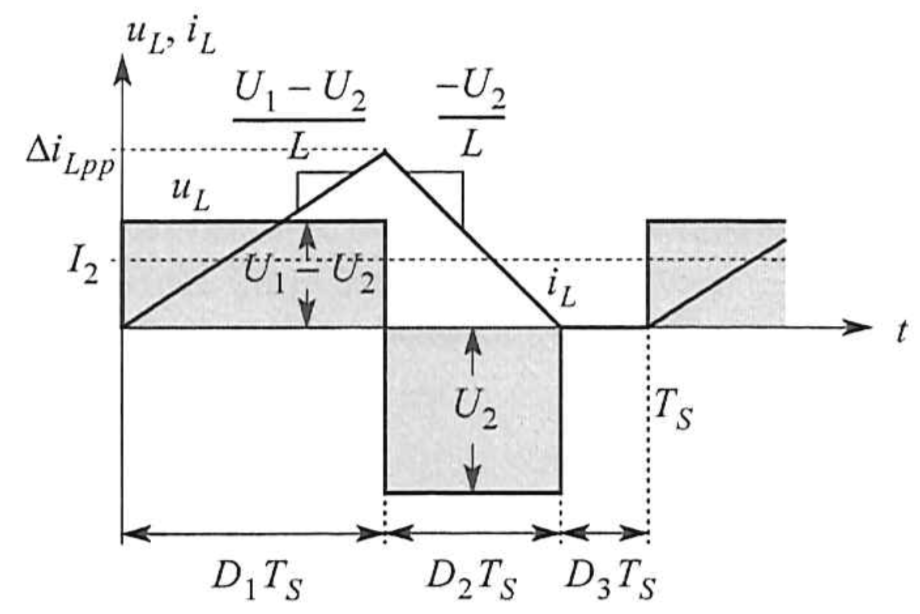
\includegraphics[width=0.4\linewidth]{img/buck/discont.png}%
  &
  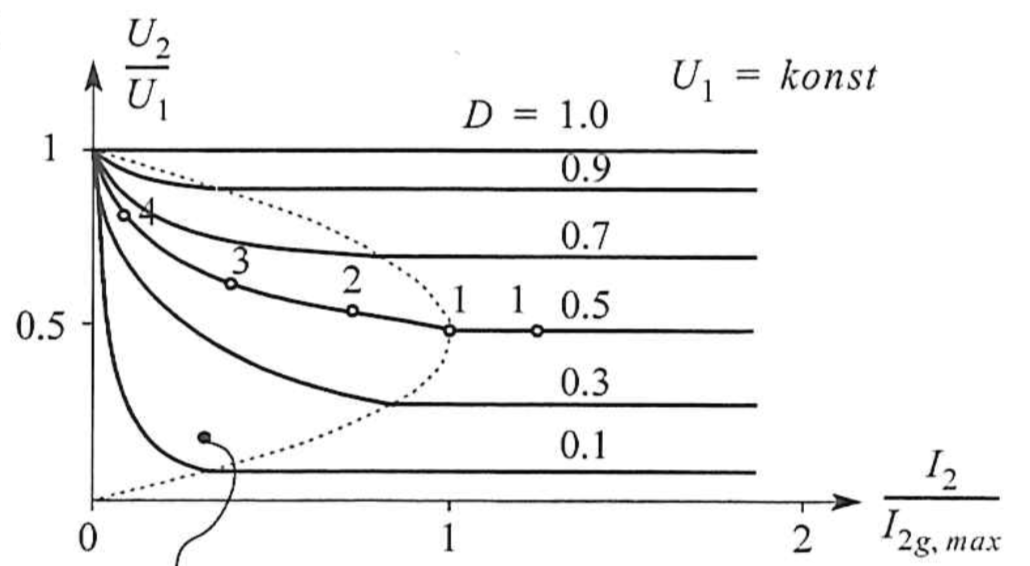
\includegraphics[width=0.4\linewidth]{img/buck/discplot.png}%
\end{tabular}

Lückender Betrieb für $I_L < I_{2g}$.

\eqn{h}{0.4\linewidth}{ I_{2g} = \frac{1}{2} \Delta i_{Lpp} = \frac{U_2}{2 \cdot L}(1-D)T_S}
\eqn{h}{0.25\linewidth}{ R_{g} = \frac{2L}{(1-D) \cdot T_S}}
\eqn{h}{0.25\linewidth}{ U_2=U_1 \frac{D_1}{D_1+D_2} }
\eqn{h}{0.3\linewidth}{ I_{2g,max}=I_{2g}|_{D=0.5} = \frac{U_1 T_S}{8L} }
\eqn{h}{0.3\linewidth}{ \frac{U_2}{U_1}=\frac{D^2}{D^2+\frac{1}{4} \frac{I_2}{I_{2g,max}} } }
\eqn{h}{0.25\linewidth}{ D = \frac{1}{2} \sqrt{\frac{I_2/I_{2g,max}}{U_1/U_2-1}} }

% -----------------------------------------------------------------------
\vfill\null
\columnbreak
\section{Hochsetzsteller}

% \begin{center}
% 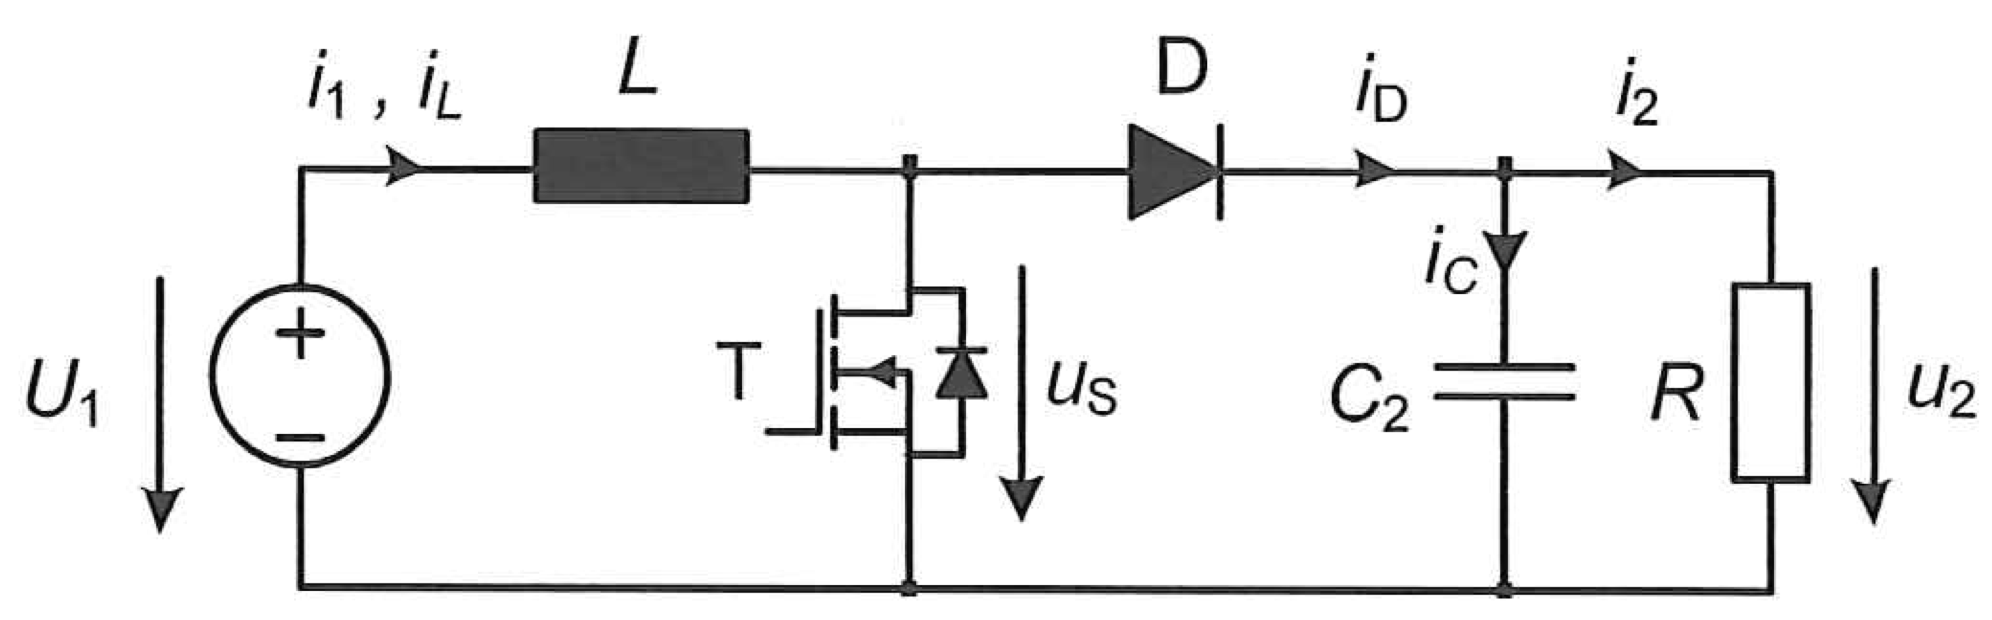
\includegraphics[width=0.8\linewidth]{img/sch_boost.png}%
% \captionof{figure}{Hochsetzsteller}%
% \end{center}

\subsection{Kontinuierlicher Stromfluss}
\begin{tabular}{c c}
  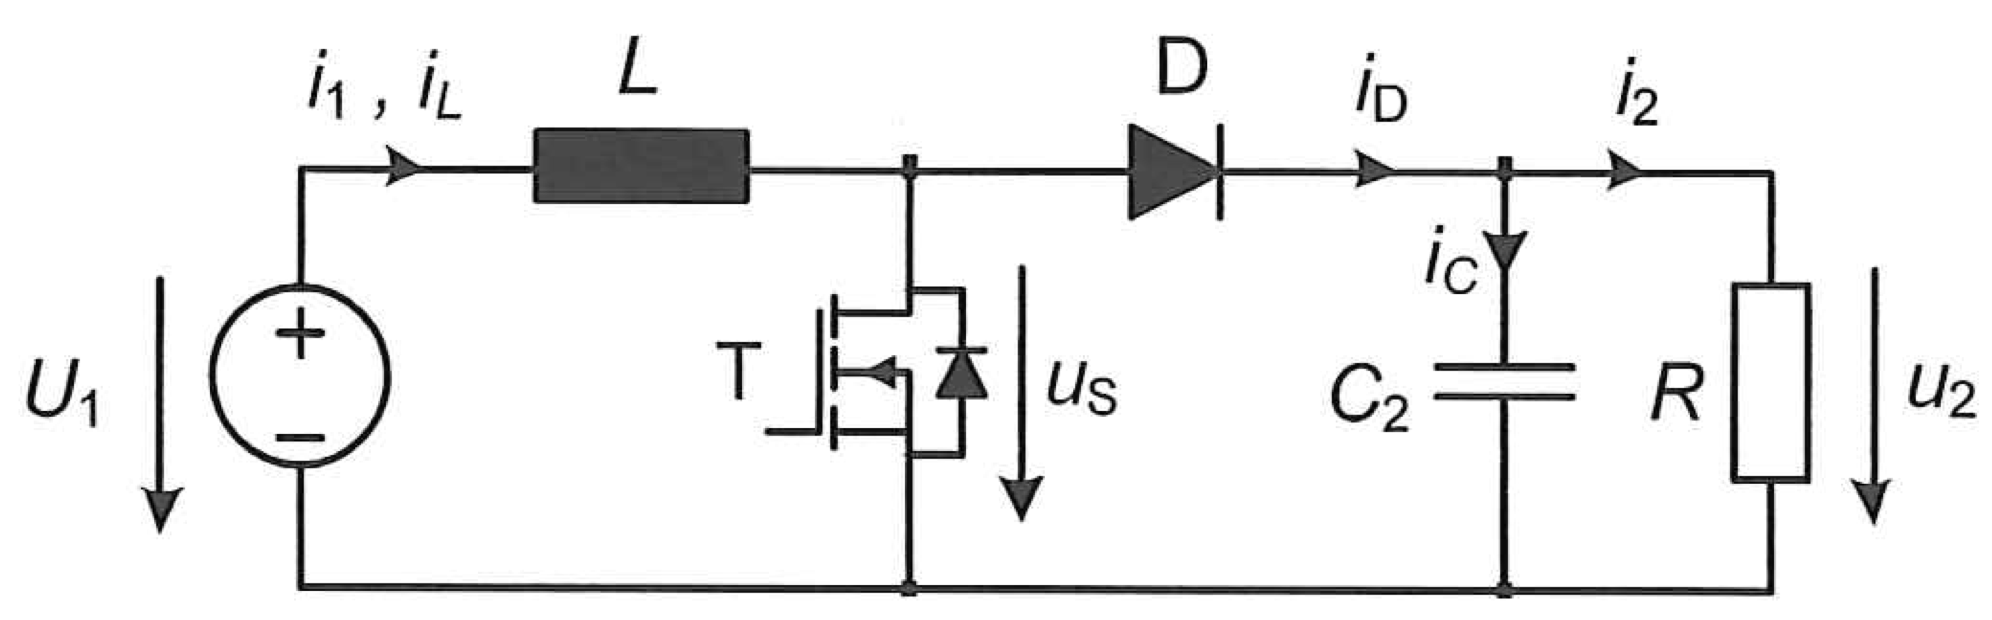
\includegraphics[width=0.4\linewidth]{img/sch_boost.png}%
  &
  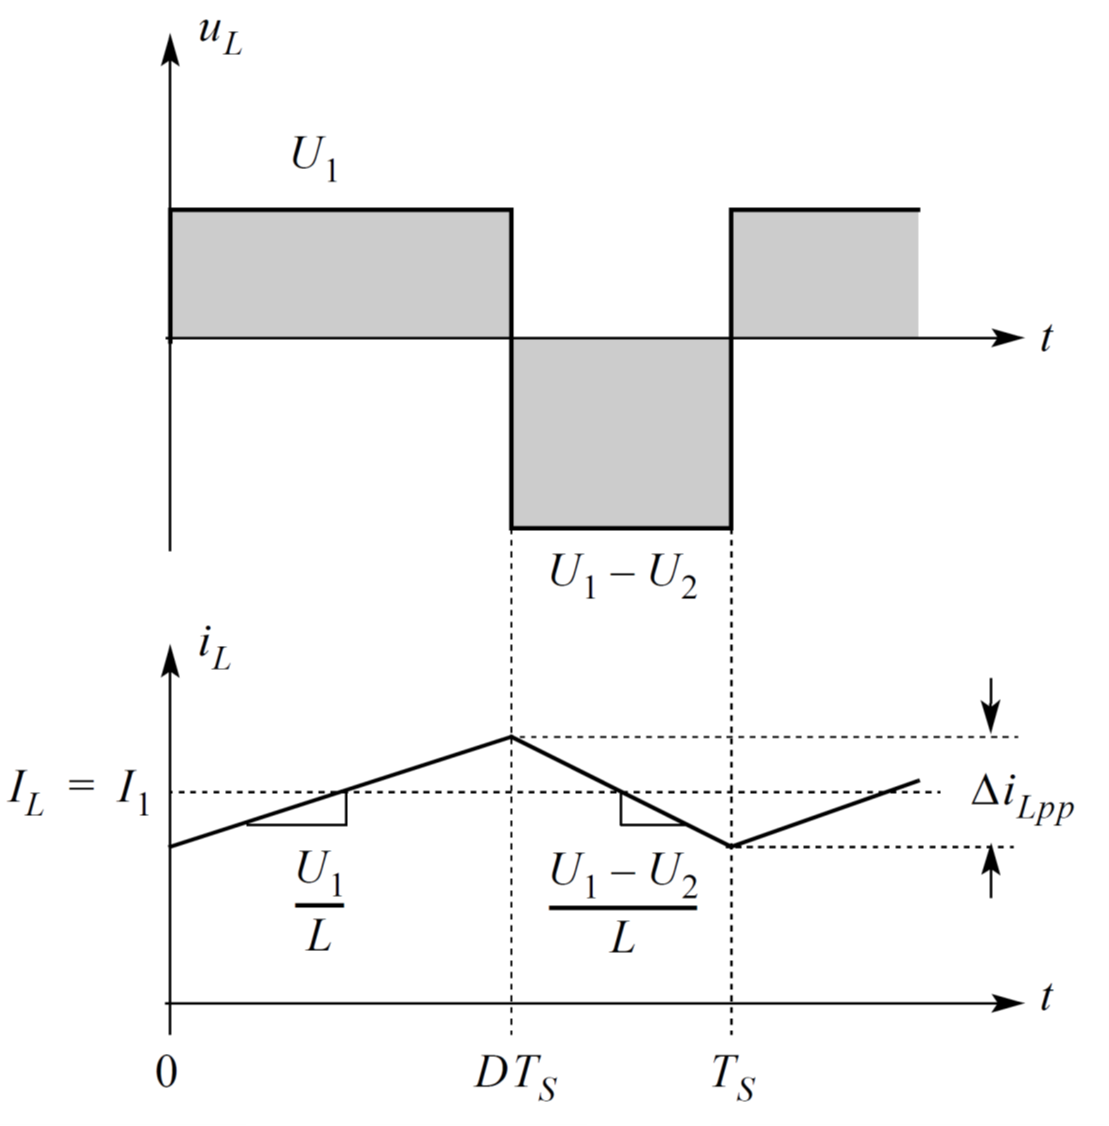
\includegraphics[width=0.4\linewidth]{img/boost/cont.png}%
\end{tabular}

\feqn{h}{0.23\linewidth}{ D = 1 - \frac{U_1}{U_2} }
\feqn{h}{0.23\linewidth}{ \frac{U_2}{U_1} = \frac{1}{1-D}}
\eqn{h}{0.23\linewidth}{ \frac{I_2}{I_1}=1-D }
\eqn{h}{0.23\linewidth}{ \Delta i_{Lpp} = \frac{U_1}{L}DT_S}

\eqn{h}{0.23\linewidth}{ \Delta U_{2pp} = \frac{U_2}{R}\frac{DT_s}{C_2} }

\subsection{Diskontinuierlicher Stromfluss}
\begin{tabular}{c c}
  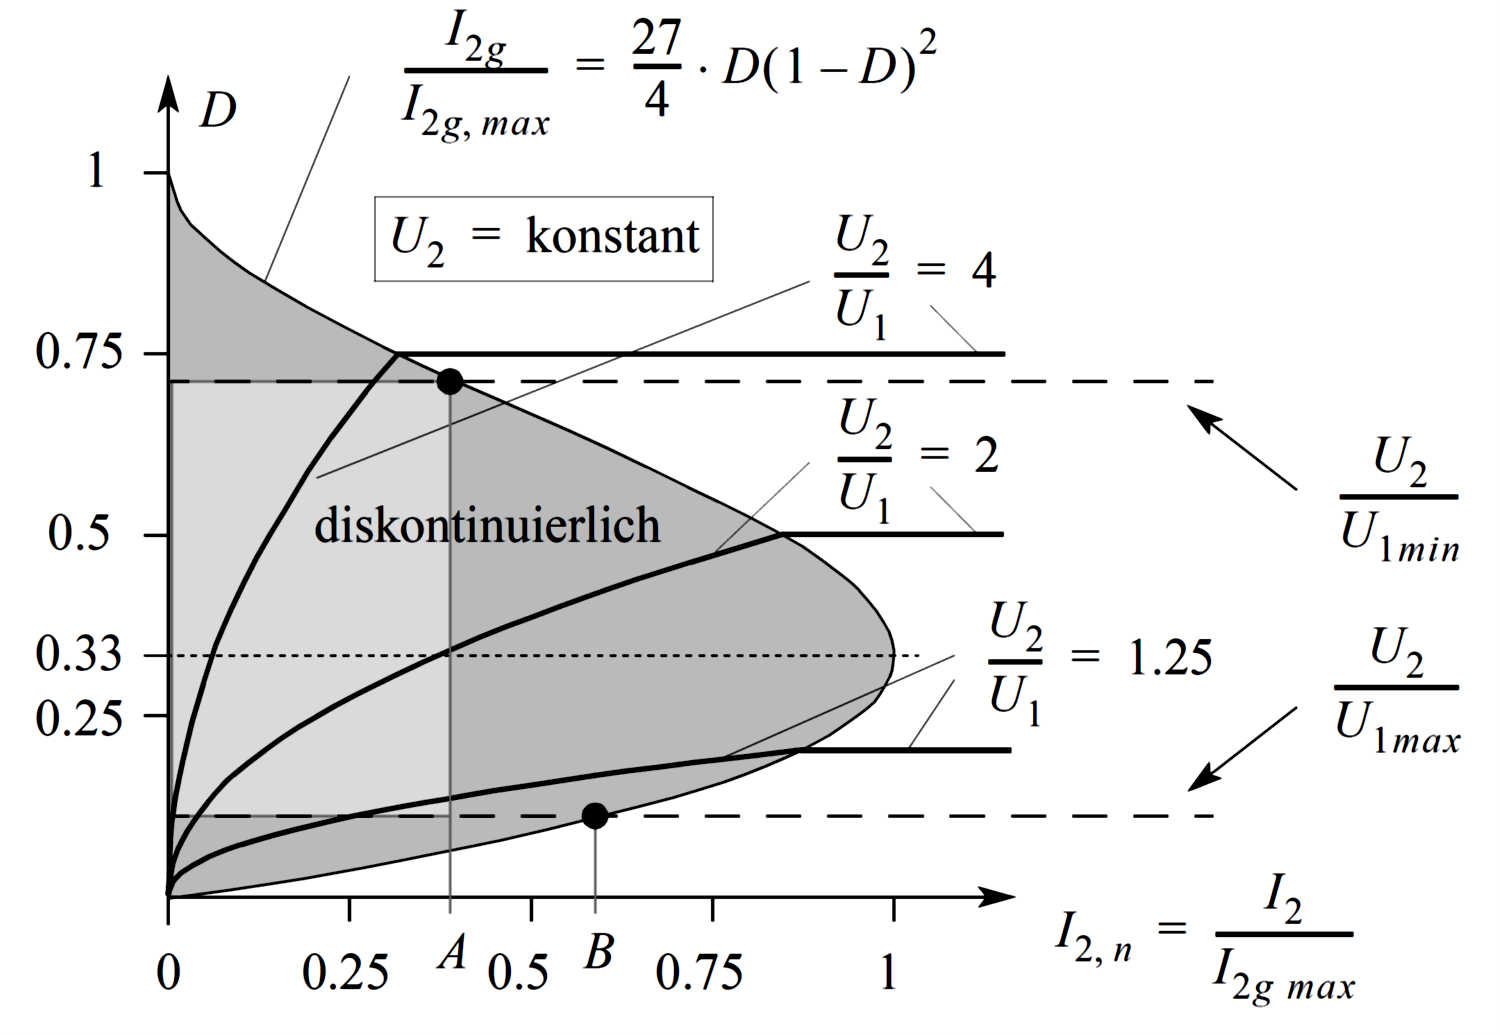
\includegraphics[width=0.4\linewidth]{img/boost/disc1.png}%
  &
  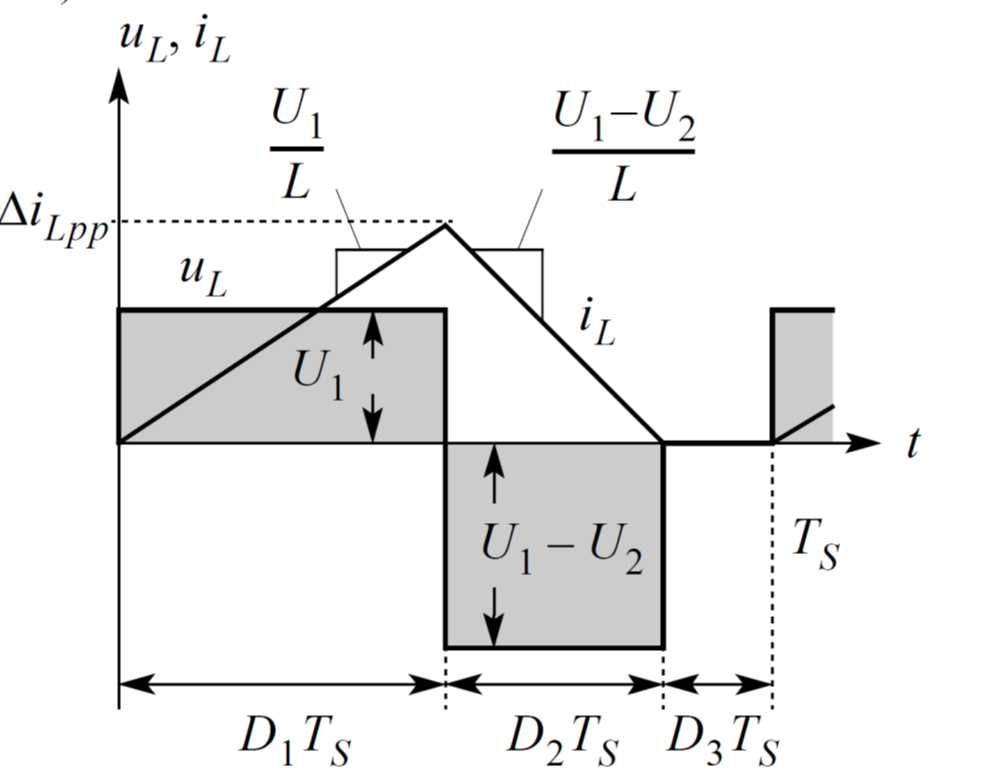
\includegraphics[width=0.4\linewidth]{img/boost/disc2.png}%
\end{tabular}

\eqn{h}{0.3\linewidth}{ I_{Lg} = \frac{1}{2} \frac{(U_2-U_1)}{L}(1-D)T_s }
\eqn{h}{0.3\linewidth}{ I_{2g} = \frac{1}{2} \frac{U_2}{L}D(1-D)^2T_s }
\eqn{h}{0.3\linewidth}{ I_{2g,max} = I_{2g}|_{D=1/3} = \frac{2}{27}\frac{U_2}{L}T_S }

\eqn{h}{0.3\linewidth}{ D= \sqrt{\frac{4}{27}\frac{U_2}{U_1} \left (\frac{U_2}{U_1}-1 \right ) \frac{I_2}{I_{2g,max}} } }
\eqn{h}{0.3\linewidth}{ I_{1g} = \frac{1}{2} \frac{U_2}{L}D(1-D)T_s }

% \eqn{h}{0.25\linewidth}{ }
% -----------------------------------------------------------------------
\vfill\null
\columnbreak
\section{Tief-Hochsetzsteller}

\begin{center}
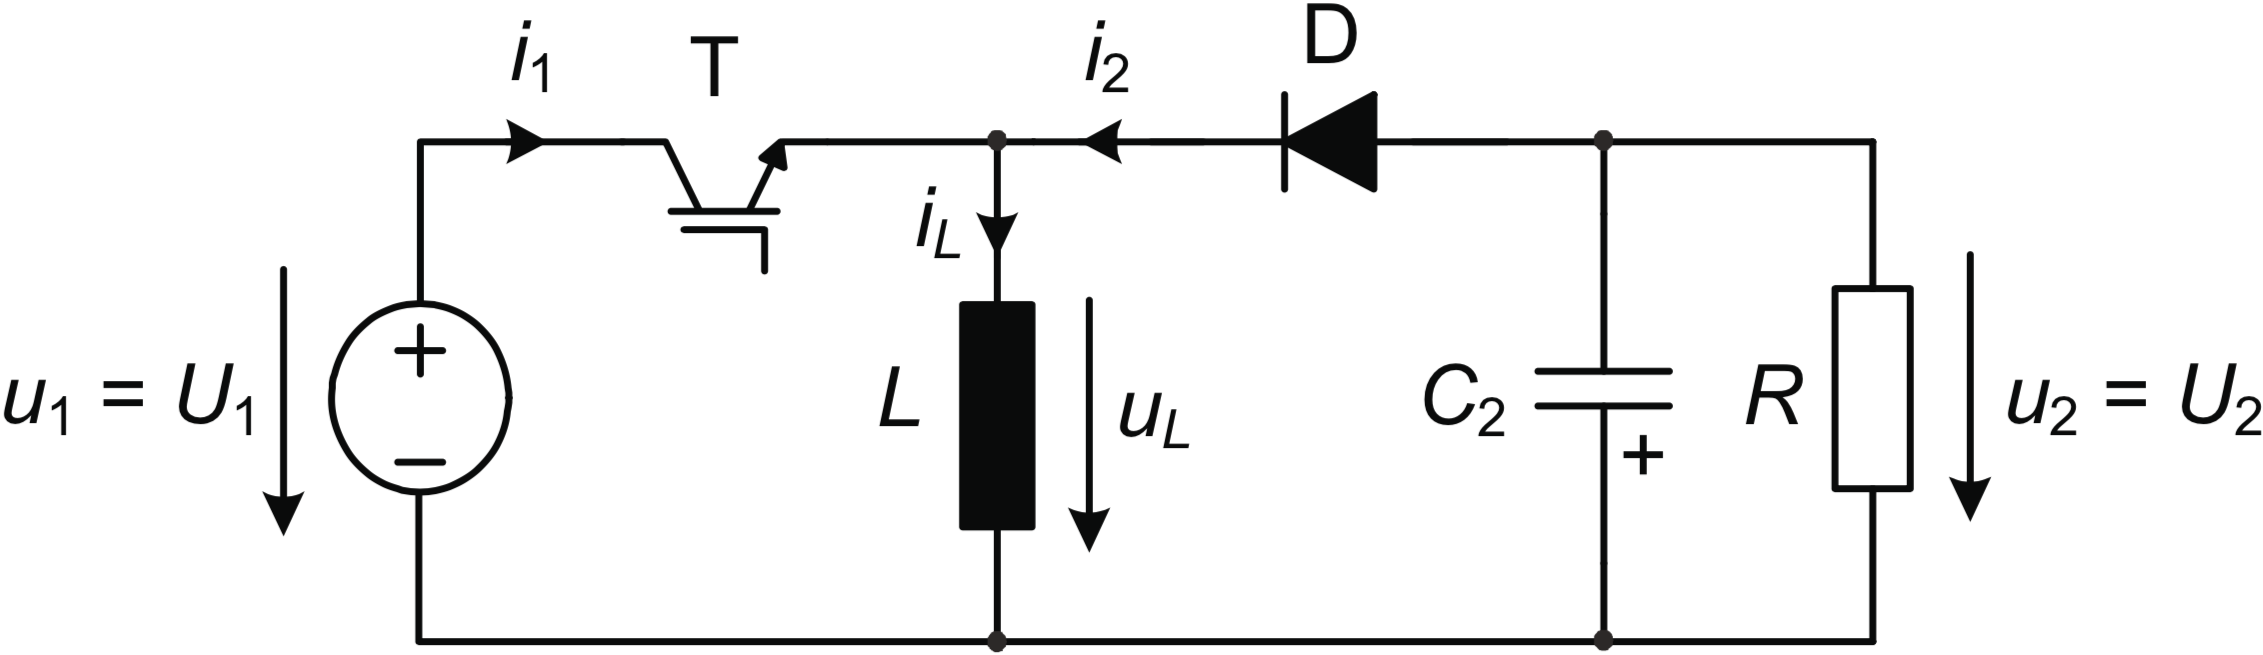
\includegraphics[width=0.8\linewidth]{img/sch_invers.png}%
% \captionof{figure}{Tief-Hochsetzsteller}%
\end{center}

\subsection{Kontinuierlicher Stromfluss}
\feqn{h}{0.23\linewidth}{ \frac{U_2}{U_1} = -\frac{D}{1-D} }
\feqn{h}{0.23\linewidth}{ D = \frac{U_2}{U_2 - U_1} }
\eqn{h}{0.23\linewidth}{ \frac{I_2}{I_1}=\frac{1-D}{D} }

\subsection{Diskontinuierlicher Stromfluss}
\begin{tabular}{c c}
  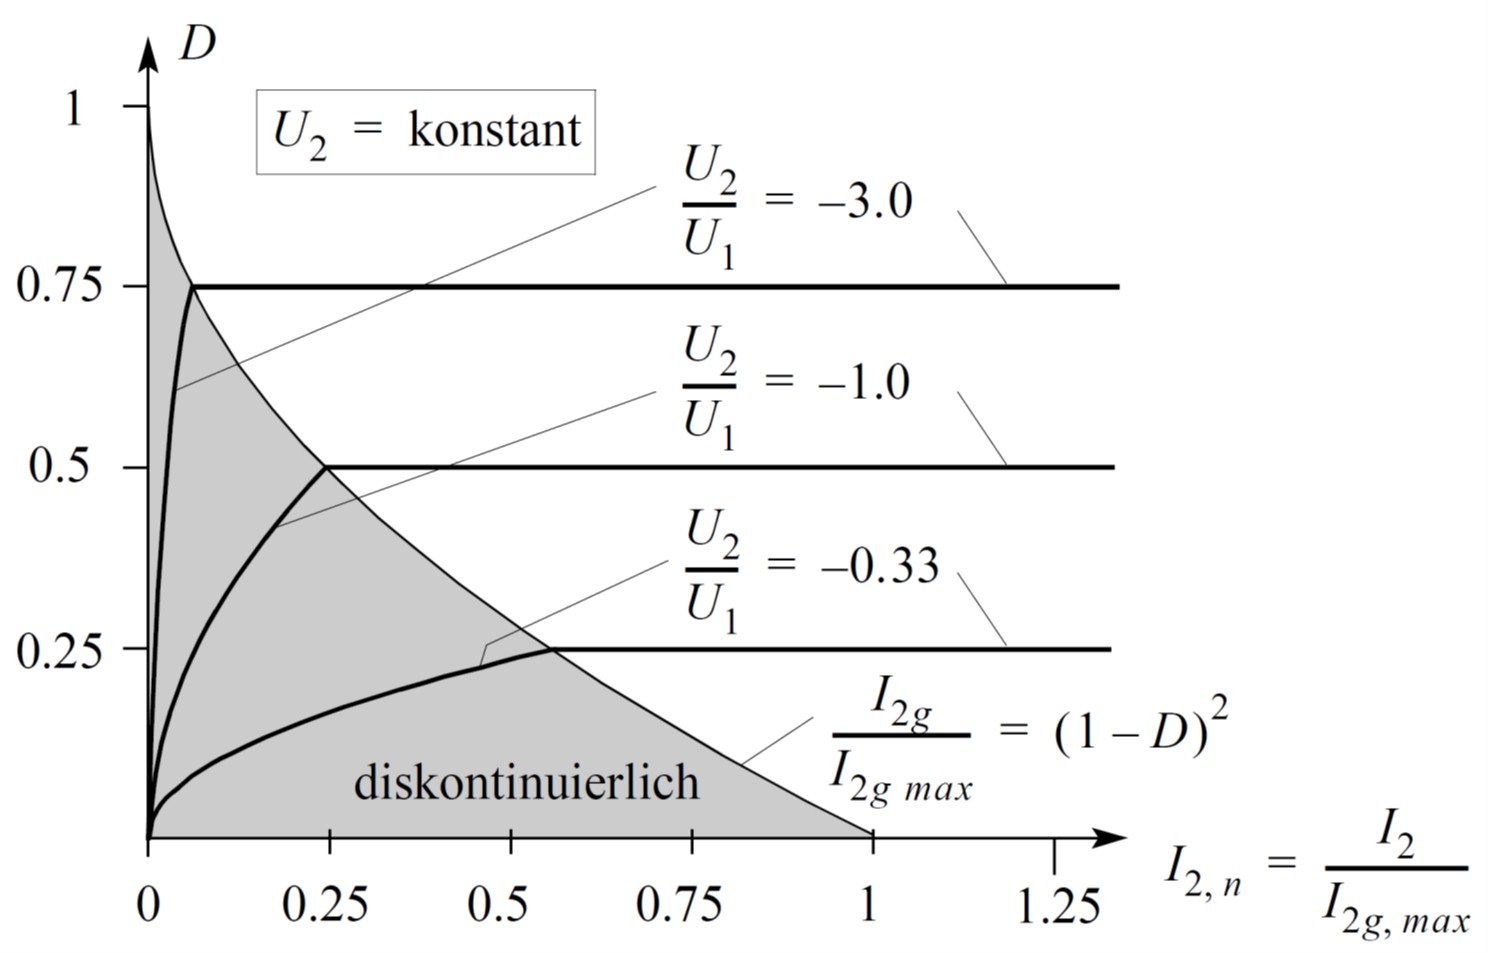
\includegraphics[width=0.4\linewidth]{img/inv/disc.png}%
  &
  % 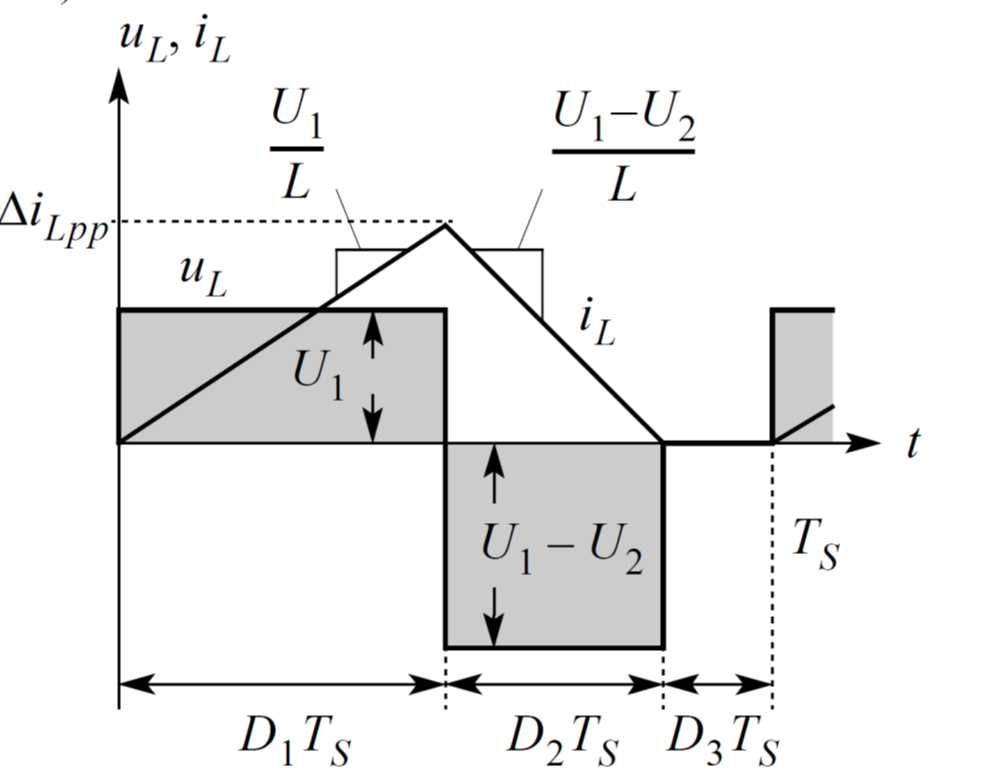
\includegraphics[width=0.4\linewidth]{img/boost/disc2.png}%
\end{tabular}

\eqn{h}{0.3\linewidth}{ I_{Lg} = \frac{1}{2} \frac{-U_2}{L}(1-D)T_s }
\eqn{h}{0.3\linewidth}{ I_{2g} = \frac{1}{2} \frac{-U_2}{L}(1-D)^2T_s }
\eqn{h}{0.3\linewidth}{ I_{2g,max} = -\frac{1}{2} \frac{U_2}{L}T_s }

\eqn{h}{0.3\linewidth}{ D = -\frac{U_2}{U_1} \sqrt{\frac{I_2}{I_{2g,max}}} }
\eqn{h}{0.65\linewidth}{ P_2 = E_L f_s = \frac{1}{2}L \cdot i_{Lmax}^2 \cdot f_s = \frac{L}{2} f_s \left( \frac{U_1 D T_s}{L} \right)^2 = \frac{U_1^2D^2}{2L}T_s }


% -----------------------------------------------------------------------
\vfill\null
\columnbreak
\section{Dioden-Gleichrichter}

\begin{tabular}{c c}
  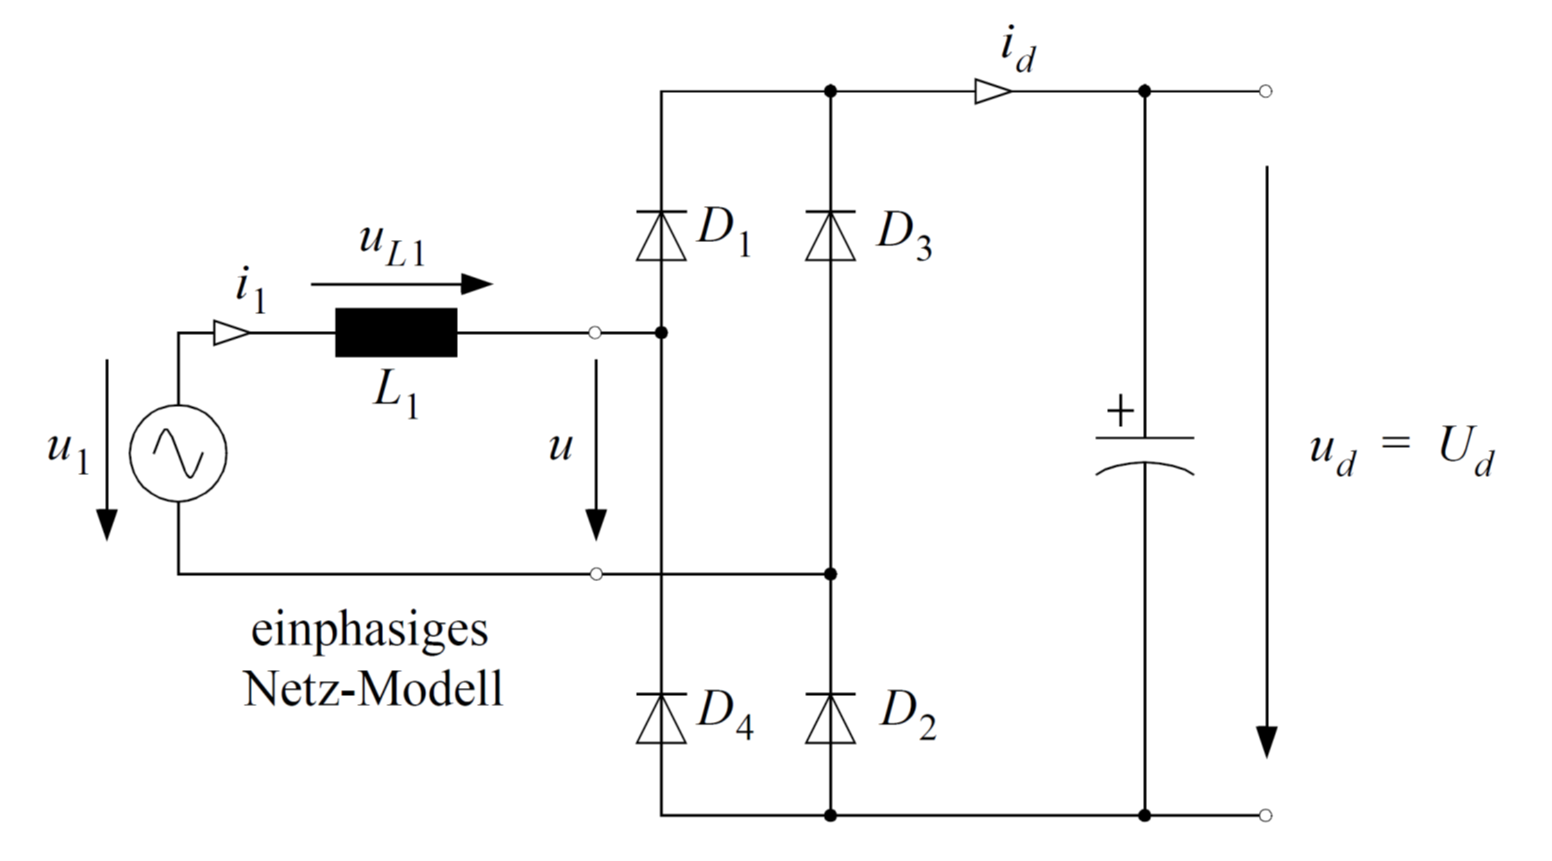
\includegraphics[width=0.49\linewidth]{img/dioderect/sch.png}%
  &
  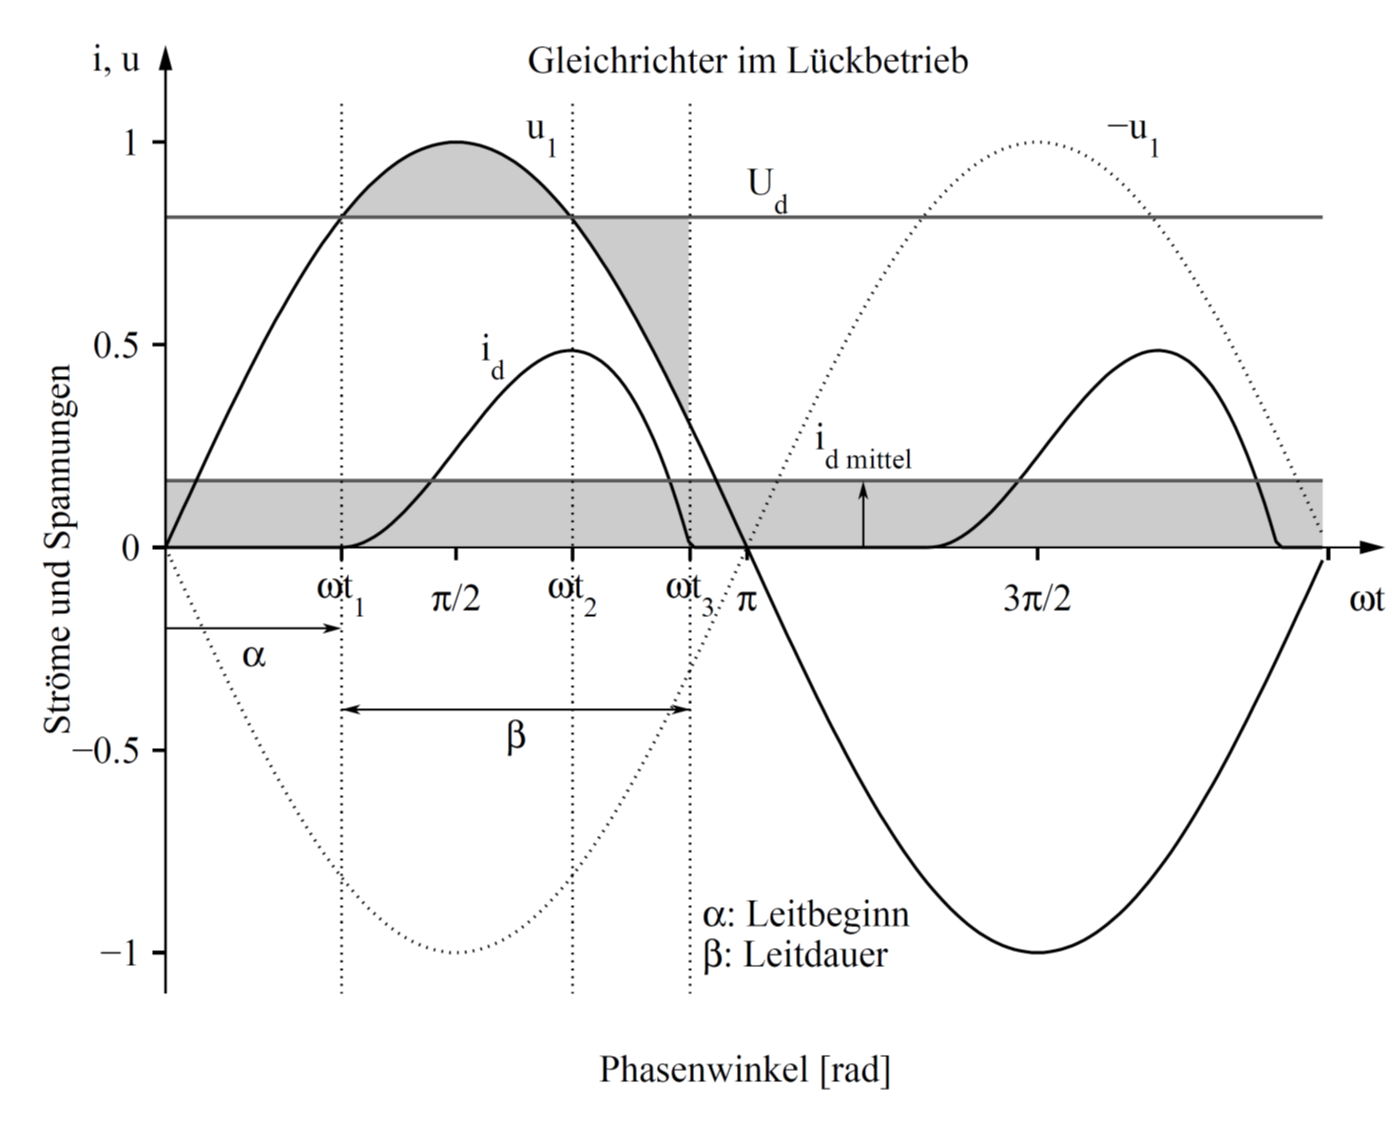
\includegraphics[width=0.49\linewidth]{img/dioderect/dia.png}%
\end{tabular}

\begin{align*}
  \alpha &= \arcsin(U_d/\hat{U_1}) = \arctan\left(\frac{1-\cos(\beta)}{\beta-\sin(\beta)}\right) & \\
  I_d &= \frac{1}{\pi}\int_{\alpha}^{\alpha+\beta}i_d(\omega t)\mathrm{d}\omega t = \frac{1}{\pi}\frac{\hat{U_1}}{\omega L_1} \left[\frac{\hat{U_1}}{U_d}(1-\cos(\beta))-\frac{U_d}{\hat{U_1}}\frac{\beta^2}{2}\right]
\end{align*}



% -----------------------------------------------------------------------
\vfill\null
\columnbreak
\section{PFC Einphasen Gleichrichter}

\begin{center}
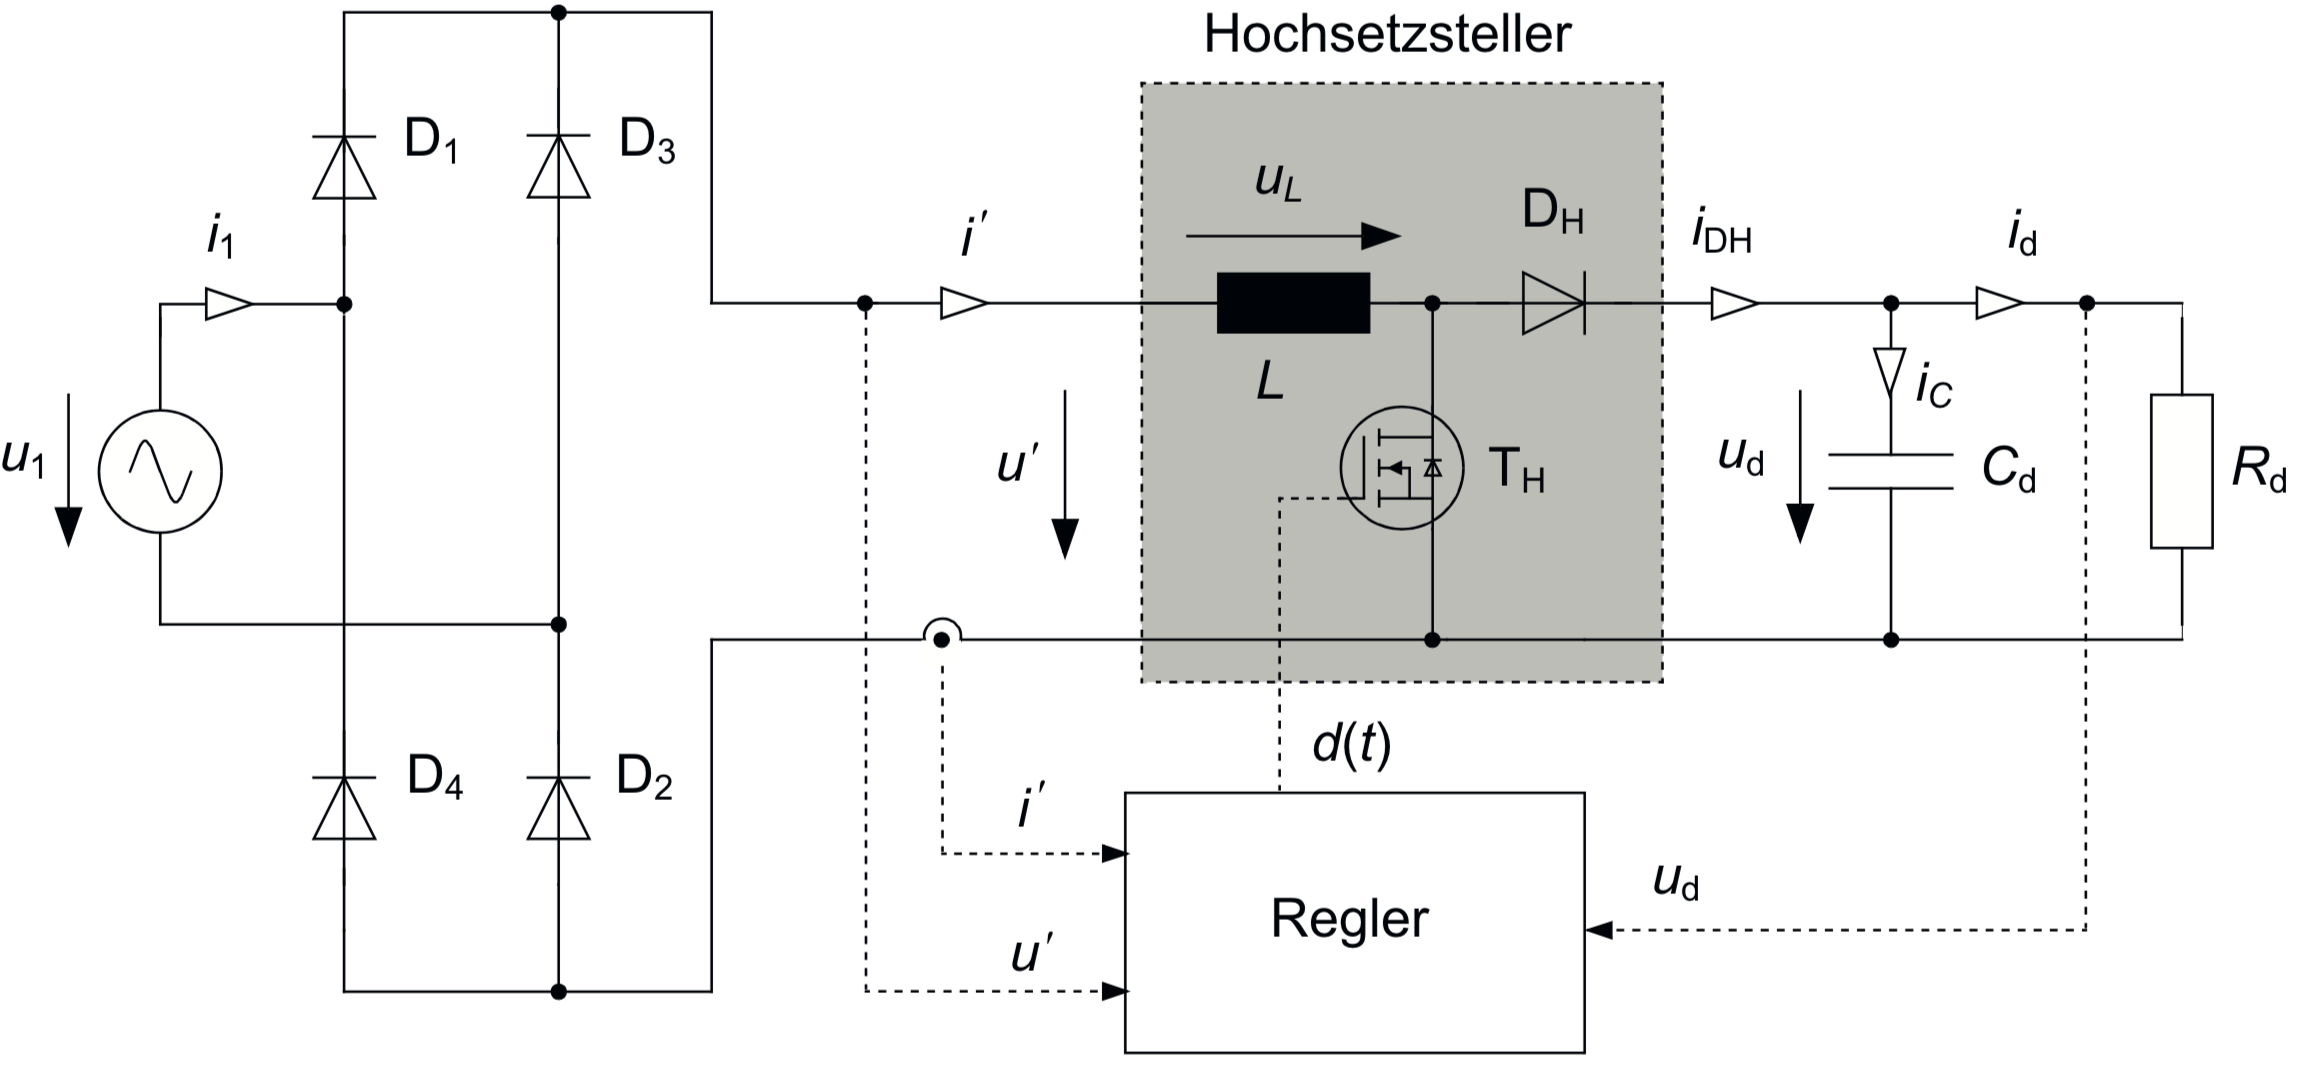
\includegraphics[width=0.8\linewidth]{img/sch_pfc.png}%
% \captionof{figure}{PFC Einphasen Gleichrichter}%
\end{center}

\subsection{Stationärer Betrieb}
L wählen mit $D(\omega t)=1$ and $U_{1,\textup{rms}}=$max. $M$: Minimales Spannungsübersetzungsverhältnis ($[M\dots\infty]$).
\begin{align*}
  D(\omega t) &= \left(1-\frac{U_1(\omega t)}{U_d}\right) & 
  \Delta i_{Lpp} (\omega t) &= D(\omega t) T_s \frac{\hat{U_1}\sin(\omega t)}{L} &
  \overline{i_L}(\omega t) &= \hat{I_1} |\sin(\omega t)| = \sqrt{2} \frac{P_d}{U_{1,\textup{rms}}}|\sin(\omega t)| \\
  \Aboxed {\overline{i_L}(\omega t) &\geq \frac{1}{2}\Delta i_{Lpp}} &
  L &\geq \frac{U_{1,\textup{rms}}^2T_s}{2P_d} &
  M &= \frac{U_d}{\sqrt{2} \cdot U_{1,\textup{rms}} }, D=\left(1-\frac{1}{M}\right) \\
  C_d &> \frac{1}{2\omega\hat{U}_{Cd}/U_d}\frac{P_d}{U_d^2} &
  \hat{U}_{Cd} &= \frac{P_d}{U_d}\frac{1}{2\omega C_d}
\end{align*}

$M$: Minimales Spannungsübersetzungsverhältnis ($[M\dots\infty]$). Das maximum des Eingangsstromrippels $\Delta i'_{pp}$ tritt auf bei $D_{\textup{max}}$. Die Phase berechnet sich durch Umformen von $D(\omega t)$.
\begin{align*}
  D_{\textup{max}} &= \begin{cases} M, & M > 2,\\ 0.5, &M < 2. \end{cases} &
  \Delta i'_{pp} &= DT_s\frac{\sqrt{2}U_{1,\textup{rms}}}{L} &
\end{align*}

\subsection{Bauteilbelastung}
\begin{align*}
  I_{\text{TH,avg}} &= \left(\frac{2}{\pi}-\frac{1}{2M}\right)\hat{I_1} &
  I_{\text{TH,rms}} &= \sqrt{\left(\frac{1}{2}-\frac{4}{3\pi M}\right)\hat{I_1^2}} &
  I_{\text{D,avg}} &= \frac{1}{2M}\hat{I_1} &
  I_{\text{D,rms}} &= \sqrt{\frac{4}{3\pi M}\hat{I_1^2}} \\
  I_{\text{Cd,rms}} &= \sqrt{\frac{1}{M}\left(\frac{4}{3\pi}-\frac{1}{4M}\right)\hat{I}_1^2} 
\end{align*}

\subsection{Toleranzbandregelung}
\eqn{h}{0.23\linewidth}{ i'_{max}=(1+k)i'^* }
\eqn{h}{0.23\linewidth}{ i'_{min}=(1-k)i'^* }
\eqn{h}{0.23\linewidth}{ \Delta i_{pp} = 2k\cdot \hat{i}'^* |sin(\omega t)| }



% -----------------------------------------------------------------------
\vfill\null
\columnbreak
\section{Netzgeführte Stromrichter}
\subsection{B6}

\begin{tabular}{b{0.49\linewidth} p{0.45\linewidth}}
  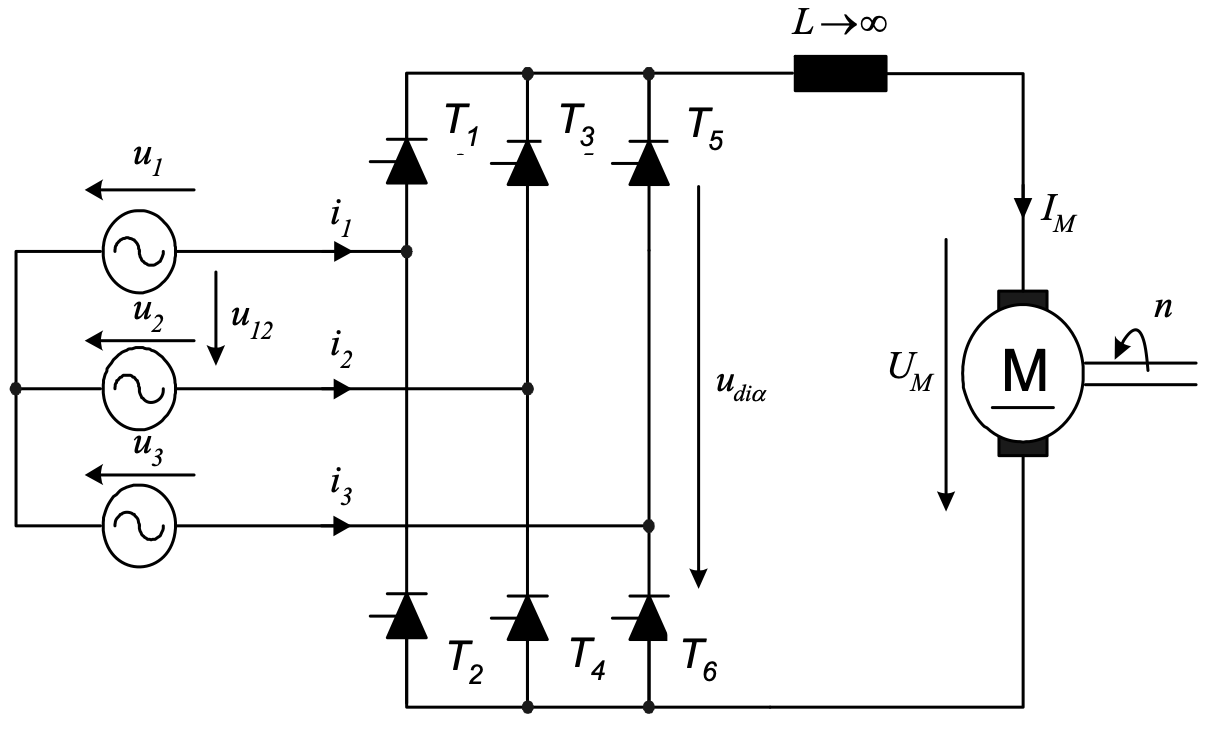
\includegraphics[width=\linewidth]{img/3p/b6.png}%
  
  Für $\alpha=\ang{0}$ ist die maximale Spannung an der Last. Für $\alpha\in[\ang{0},\ang{90}]$ wird die Spannung immer kleiner. Für $\alpha=\ang{90}$ ist die Spannung an der Last $=0$. Mit $\alpha\in[\ang{90},\ang{180}]$ bleibt die Stromrichtung dieselbe aber die Spannung wechselt das Vorzeiechen. Es wird Leistung zurückgespeist.
  
  \textbf{Zeichnen:} Ab Schnitt von $u_1,u_2$ $\alpha$ oben und unten abtragen.

  $Q$: Grundschwingungsblindleistung
  &
  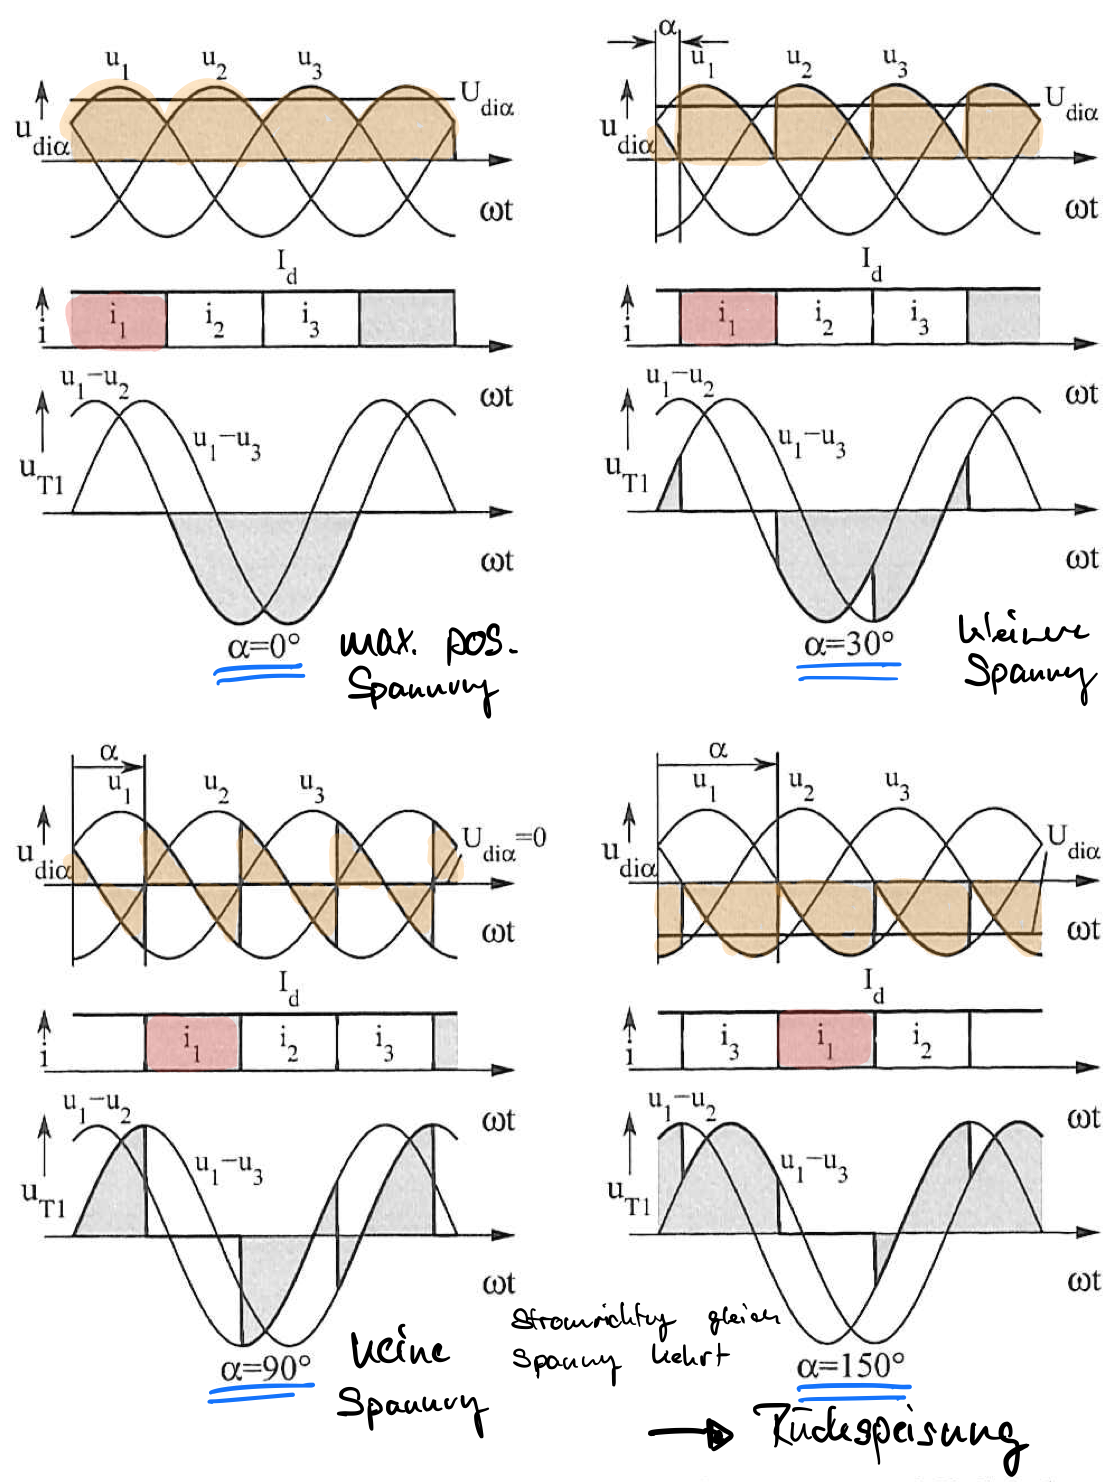
\includegraphics[width=\linewidth]{img/3p/graph.png}%
\end{tabular}


\begin{align*}
  U_{\textup{di,}\alpha} &= \frac{3\sqrt{6}}{\pi} U_1\cos{\alpha} &
  I_{1,\textup{rms}} &= \sqrt{\frac{2}{3}}I_M &
  \hat{I}_{1,(1)} &= \frac{1}{\pi}\Int_0^{2\pi}i_1(t)\cos(\omega t) \mathrm{d}\omega t = \frac{2\sqrt{3}}{\pi}I_d \\
  Q_1 &= U_1I_{1,(1)}\sin(\alpha) &
\end{align*}


\subsection{Netzgeführte Stromrichter}

\begin{tabular}{b{0.69\linewidth} p{0.29\linewidth}}
  \begin{center}
  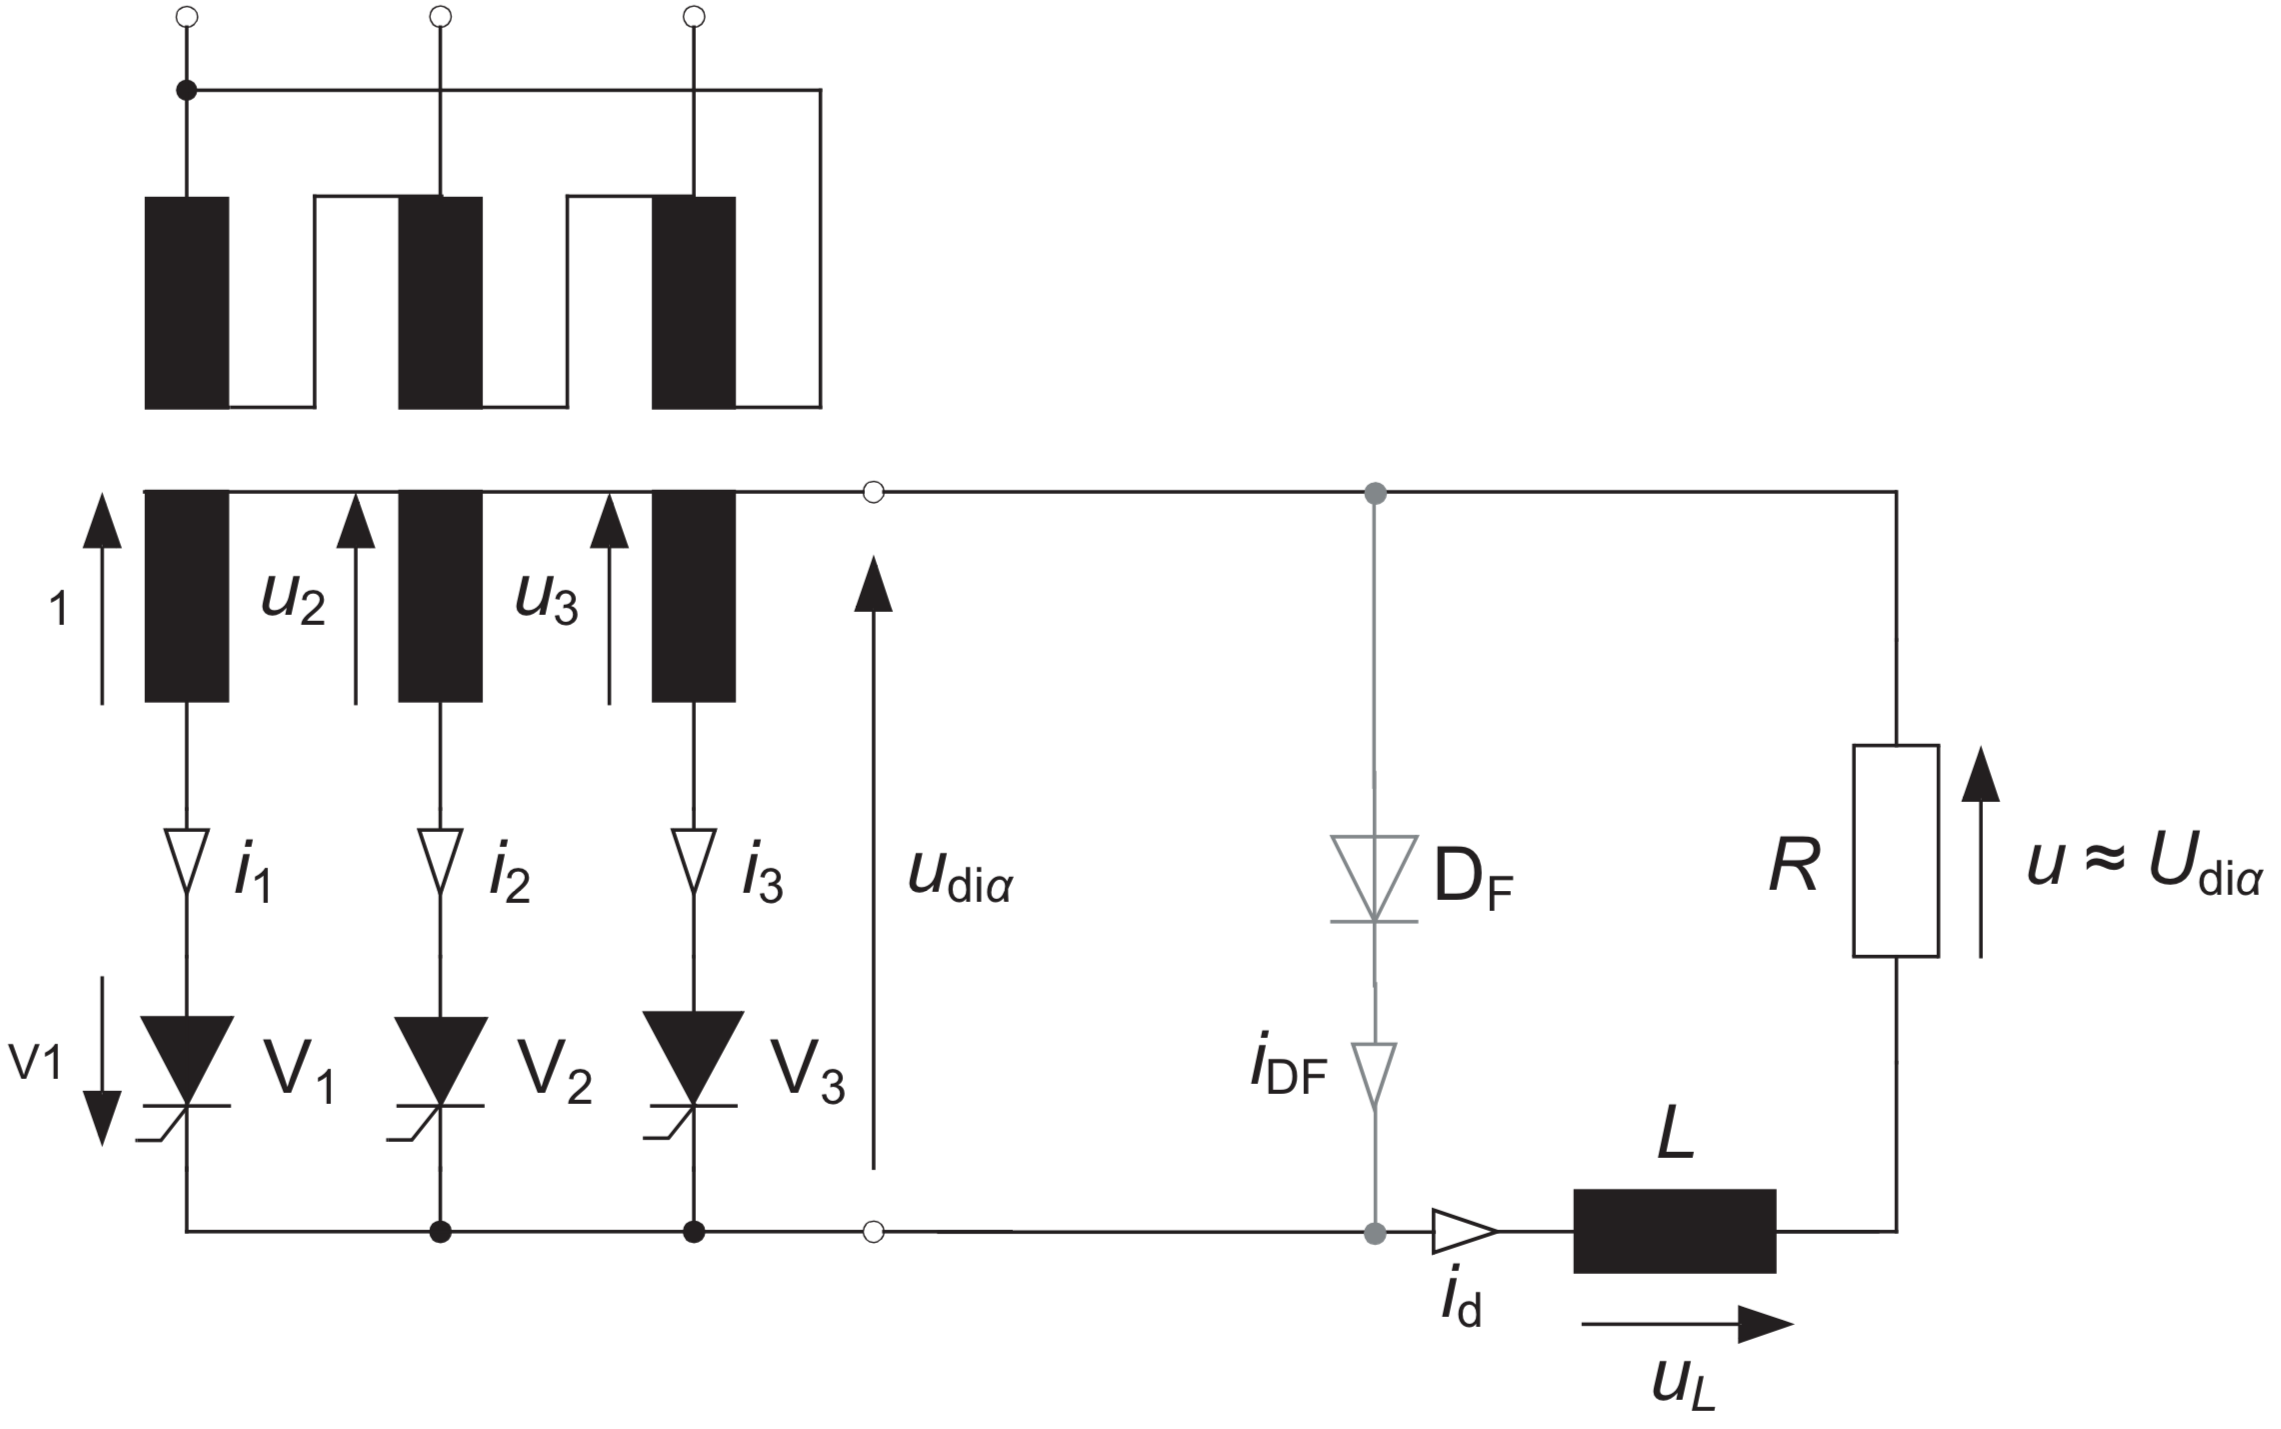
\includegraphics[width=0.5\linewidth]{img/sch_netz_dreiphase.png}%
  \end{center}
    {\begin{align*}
      % U&=RI
      U_{\textup{di,}\alpha}&=\frac{3}{\pi}\sqrt{\frac{3}{2}} U_1 \cos(\alpha) &
      \frac{U_{\textup{di,}\alpha}}{U_{\textup{di,}0}} &= \cos(\alpha)
    \end{align*}}

    Lückender Betrieb (für $\ang{30}<\alpha<\ang{150}$):
    {\begin{align*}
      U_{\textup{di,}\alpha}&=\frac{3}{\pi}\sqrt{\frac{3}{2}} U_1 \frac{1-\sin(\alpha-\pi/3)}{2\sin(\pi/3)}
    \end{align*}}
  &
  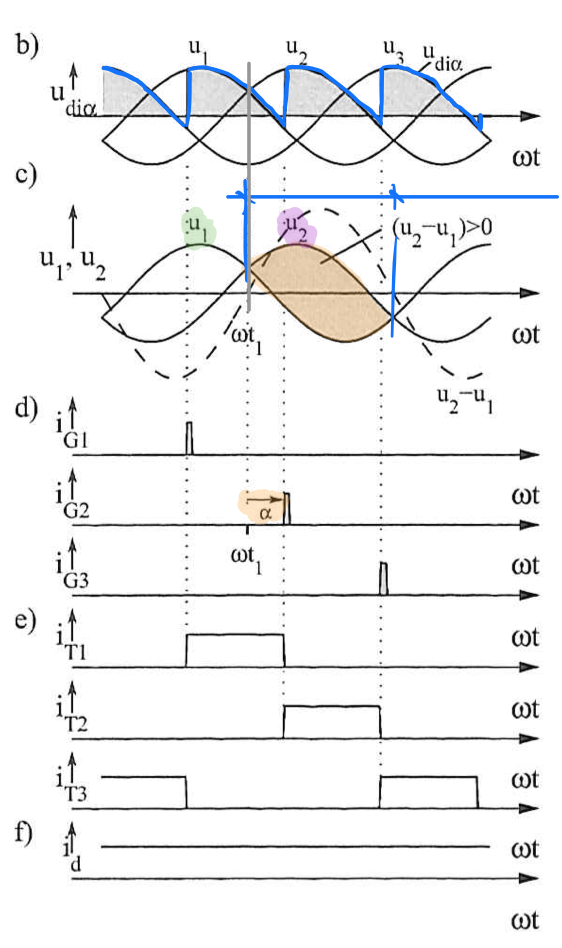
\includegraphics[width=\linewidth]{img/3p/graph2.png}%
\end{tabular}
  


% -----------------------------------------------------------------------
\vfill\null
\columnbreak
\section{Induktivität Dimensionierung}

\begin{minipage}[h]{0.6\linewidth}
  \begin{tabular}{l l l |}
    $A_n$   & Wicklungsfenster      & $mm^2 = 10^{-6}m^2$ \\
    $A_e$   & Eisenquerschnitt      & $mm^2 = 10^{-6}m^2$ \\
    $B_S$   & Sättigungsinduktion   & $\approx 0.3T$ \\
    $k_f$   & Füllfaktor            & $\approx 0.5$ \\
    $S$     & zulässige Stromdichte & $\approx 5\frac{A}{mm^2}=5\cdot10^6\frac{A}{m^2}$ \\
    $d$     & Luftspalt             & $m$ \\
    $\mu_0$ & Vacuum permeability   & $1.256\cdot10^{-6}Vs/(Am)$
  \end{tabular}
\end{minipage}
\begin{minipage}[h]{0.3\linewidth}
\textbf{Vorgehen}
  \begin{enumerate}
    \item Berechne Flächenprodukt $A_e A_n$
    \item Suche Kern mit grösserem Flächenprodukt
    \item Berechne N
    \item Berechne Luftspalt
  \end{enumerate}
\end{minipage}


\eqn{h}{0.23\linewidth}{ A_e > \frac{L\hat{I}}{B_S N} }
\eqn{h}{0.23\linewidth}{ A_n > \frac{NI_{\textup{rms}}}{k_f S} }
\eqn{h}{0.23\linewidth}{ A_e A_n = \frac{L \hat{I} I_{\textup{rms}}}{B_S k_f S} }
\eqn{h}{0.23\linewidth}{ \frac{L \hat{I} }{A_e S} < N < \frac{A_n k_f S}{I_{\textup{rms}}} }

\eqn{h}{0.23\linewidth}{ A_{cu} S = I_{max} }
\eqn{h}{0.23\linewidth}{ d = \frac{R_{tot}\mu_0 A_e}{2} = \frac{N^2 \mu_0 A_e}{2L} }


% -----------------------------------------------------------------------
\vfill\null
\columnbreak
\section{Trafo Dimensionierung}

\begin{minipage}[h]{0.6\linewidth}
  \begin{tabular}{l l l |}
    $A_n/A_w$   & Wicklungsfenster      & $mm^2 = 10^{-6}m^2$ \\
    $A_e$   & Eisenquerschnitt      & $mm^2 = 10^{-6}m^2$ \\
    $B_S$   & Sättigungsinduktion   & $\approx 0.3T$ \\
    $k_f$   & Füllfaktor            & $\approx 0.5$ \\
    $S$     & zulässige Stromdichte & $\approx 5\frac{A}{mm^2}=5\cdot10^6\frac{A}{m^2}$ \\
    $d$     & Luftspalt             & $m$ \\
    $\mu_0$ & Vacuum permeability   & $1.256\cdot10^{-6}Vs/(Am)$
  \end{tabular}
\end{minipage}
\begin{minipage}[h]{0.3\linewidth}
\textbf{Vorgehen}
  \begin{enumerate}
    \item Berechne Flächenprodukt $A_e A_n$
    \item Suche Kern mit grösserem Flächenprodukt
    \item Berechne N
    \item Berechne Luftspalt
  \end{enumerate}
\end{minipage}

\textbf{Dimensionierung}
\begin{align*}
  A_EA_W &= \frac{U_1}{f_p}\frac{D}{B_S}\frac{2\frac{I_{1,avg}}{\sqrt{D}}}{k_f S_{\textup{rms}}} \approx \frac{U_1I_{1,avg}}{f_p} & 
  \left\lceil \frac{\hat{\Psi}_{phys}}{A_EB_{sat}} \right\rceil &\leq N \leq
  \left\lfloor \frac{1}{2}\frac{S_{\textup{rms}}}{I_{p,\textup{rms}}k_f A_w} \right\rfloor &
  \hat{\Psi}_{phys} &= \max\int_{T}^{}u_p(t)\mathrm{d}t
\end{align*}
Typisch: $N$ das Minimum nehmen. Falls kein $N$ wählbar ist, anderen Kern wählen.

\textbf{Hauptinduktivität}
\begin{align*}
  L_h &= N_p^2\frac{1}{R_m} = \frac{N_p^2A_e\mu_r\mu_0}{l_e} & l_e \quad \text{Mittlere Wdg.länge}
\end{align*}

\textbf{Verluste}
\begin{align*}
  P_{cu} &= R_{cu,p}I_{1,\textup{rms}}^2+R_{cu,s}I_{2,\textup{rms}}^2 &
  R_{cu} &= \rho_{cu} \frac{l_{cu}}{A_{cu}} &
  l_{cu} &= N\cdot l_n &
  A_{cu} &= \frac{I_{\textup{rms}}}{S_{\textup{rms}}}
\end{align*}

\textbf{Streuung}
Problem: Nicht alle Induktionslinien von einer Seite sind mit der anderen Seite verkettet. 

\begin{minipage}[h]{0.6\linewidth}
  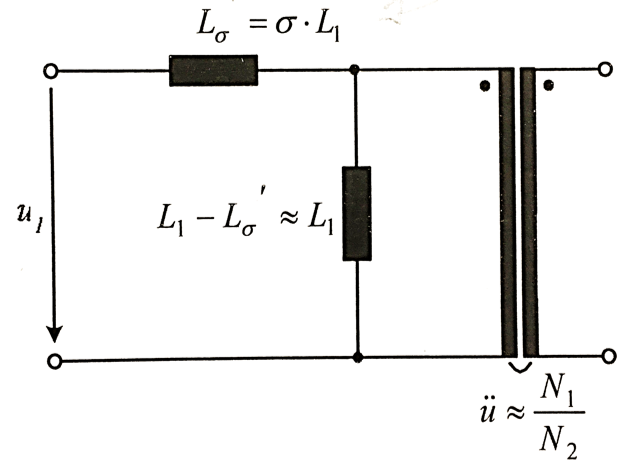
\includegraphics[width=\linewidth]{img/trafo/trafo_tech_esb.png}%
\end{minipage}
\begin{minipage}[h]{0.3\linewidth}\begin{align*}
      &\oint_{\partial A}\vec{H}\mathrm{d}\vec{s} = H\cdot h \\
      W_m &= \frac{1}{2}\mu_0 \iiint_V H^2\mathrm{d}V
    \end{align*}
\end{minipage}
% -----------------------------------------------------------------------
\vfill\null
\columnbreak
\section{Sperrwandler}

\begin{tabular}{b{0.30\linewidth} b{0.61\linewidth}}
  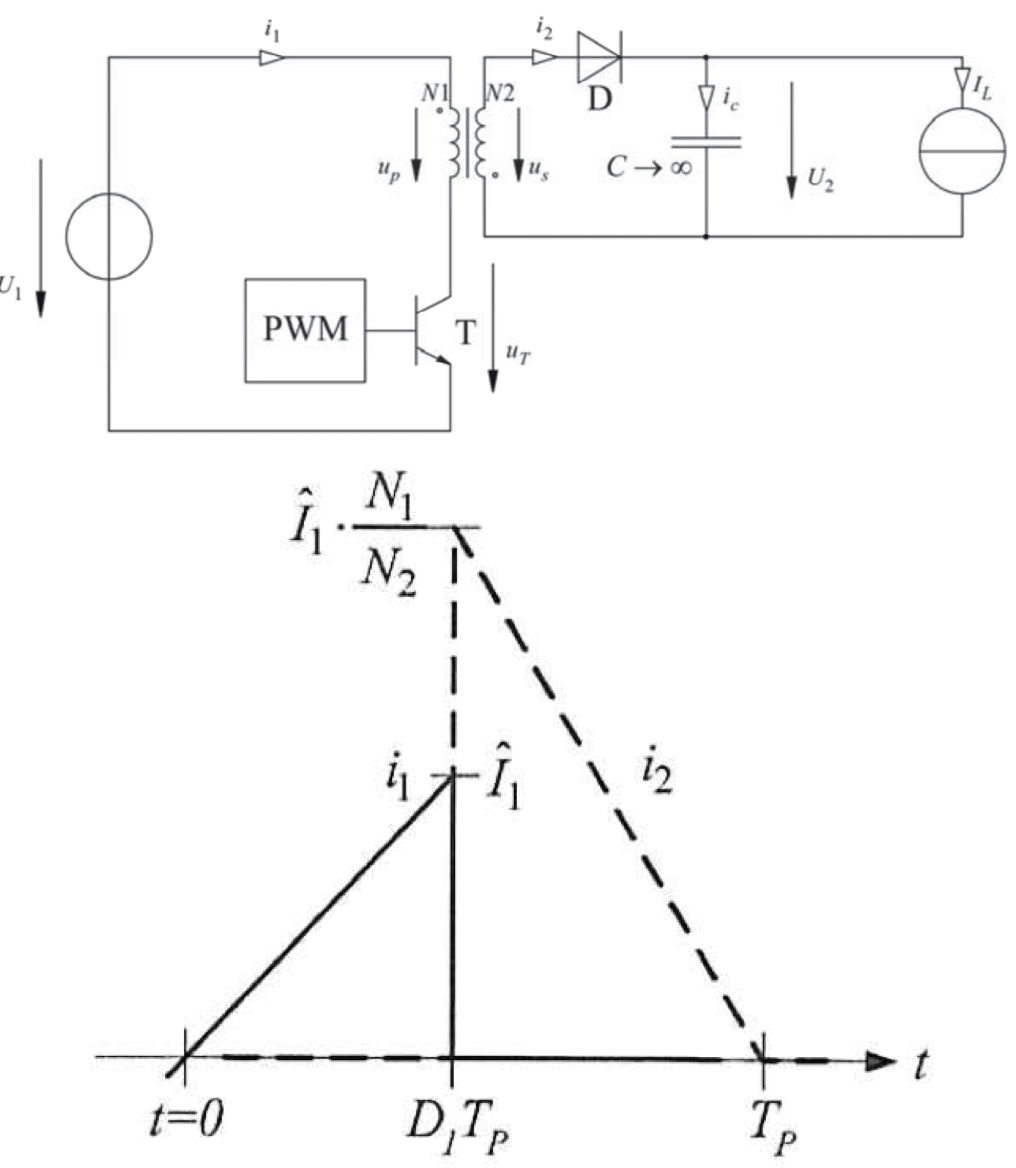
\includegraphics[width=1.0\linewidth]{img/flyback/sch.png}%
  {\begin{align*}
    \hat{I}_1 &= \frac{U_1}{L_1}D_1T_p & \hat{I}_1N_1 &= \hat{I}_2N_2
  \end{align*}}
  &
  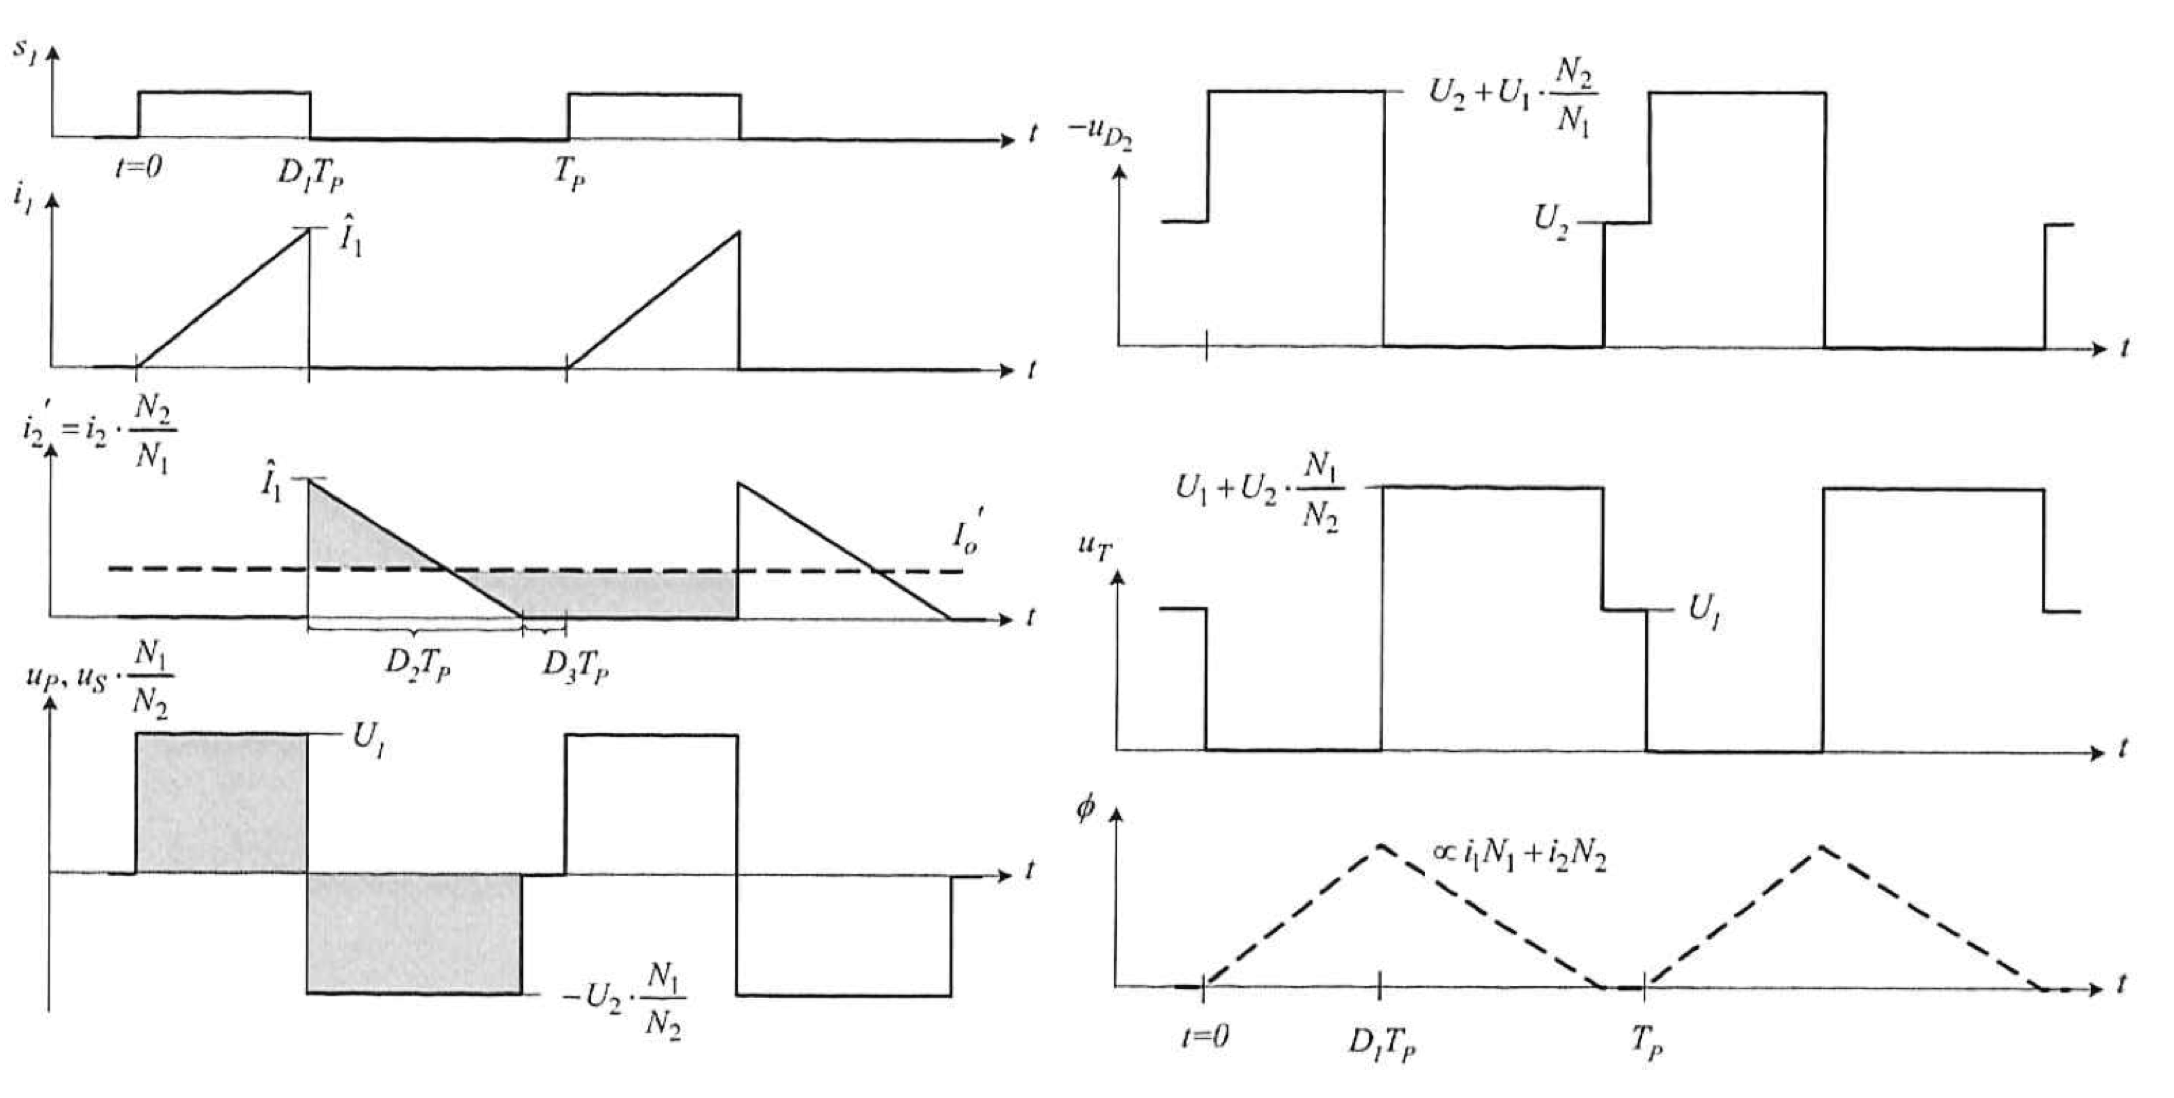
\includegraphics[width=\linewidth]{img/flyback/g1g2.png}%

  Wird üblicherweis im diskontinuierlichen Betrieb betrieben. Die Leistung entspricht der pro Taktperiode gepseicherten Energie im Kern der Induktivität (Ersatzschaltbild).
  {\begin{align*}
    P_2 &= \frac{W_m}{T_p} = \frac{1}{2}\frac{U_1^2}{L_1}D_1^2T_p &
    W_m &= \frac{1}{2}L_1\hat{I}_1 &
    \hat{I}_1 &= \frac{U_1}{L_1}D_1T_p
  \end{align*}}

\end{tabular}
  
\subsection{Kontinuierlicher Betrieb / Lückgrenze}
\begin{align*}
  D_1 &= \frac{U_2N_1}{U_2N_1 + U_1N_2} &
  \frac{U_2}{U_1} &= \frac{N_2}{N_1}\frac{D_1}{1-D_1}
\end{align*}

% -----------------------------------------------------------------------
\vfill\null
\columnbreak
\section{Durchflusswandler}

\begin{tabular}{b{0.30\linewidth} b{0.61\linewidth}}
  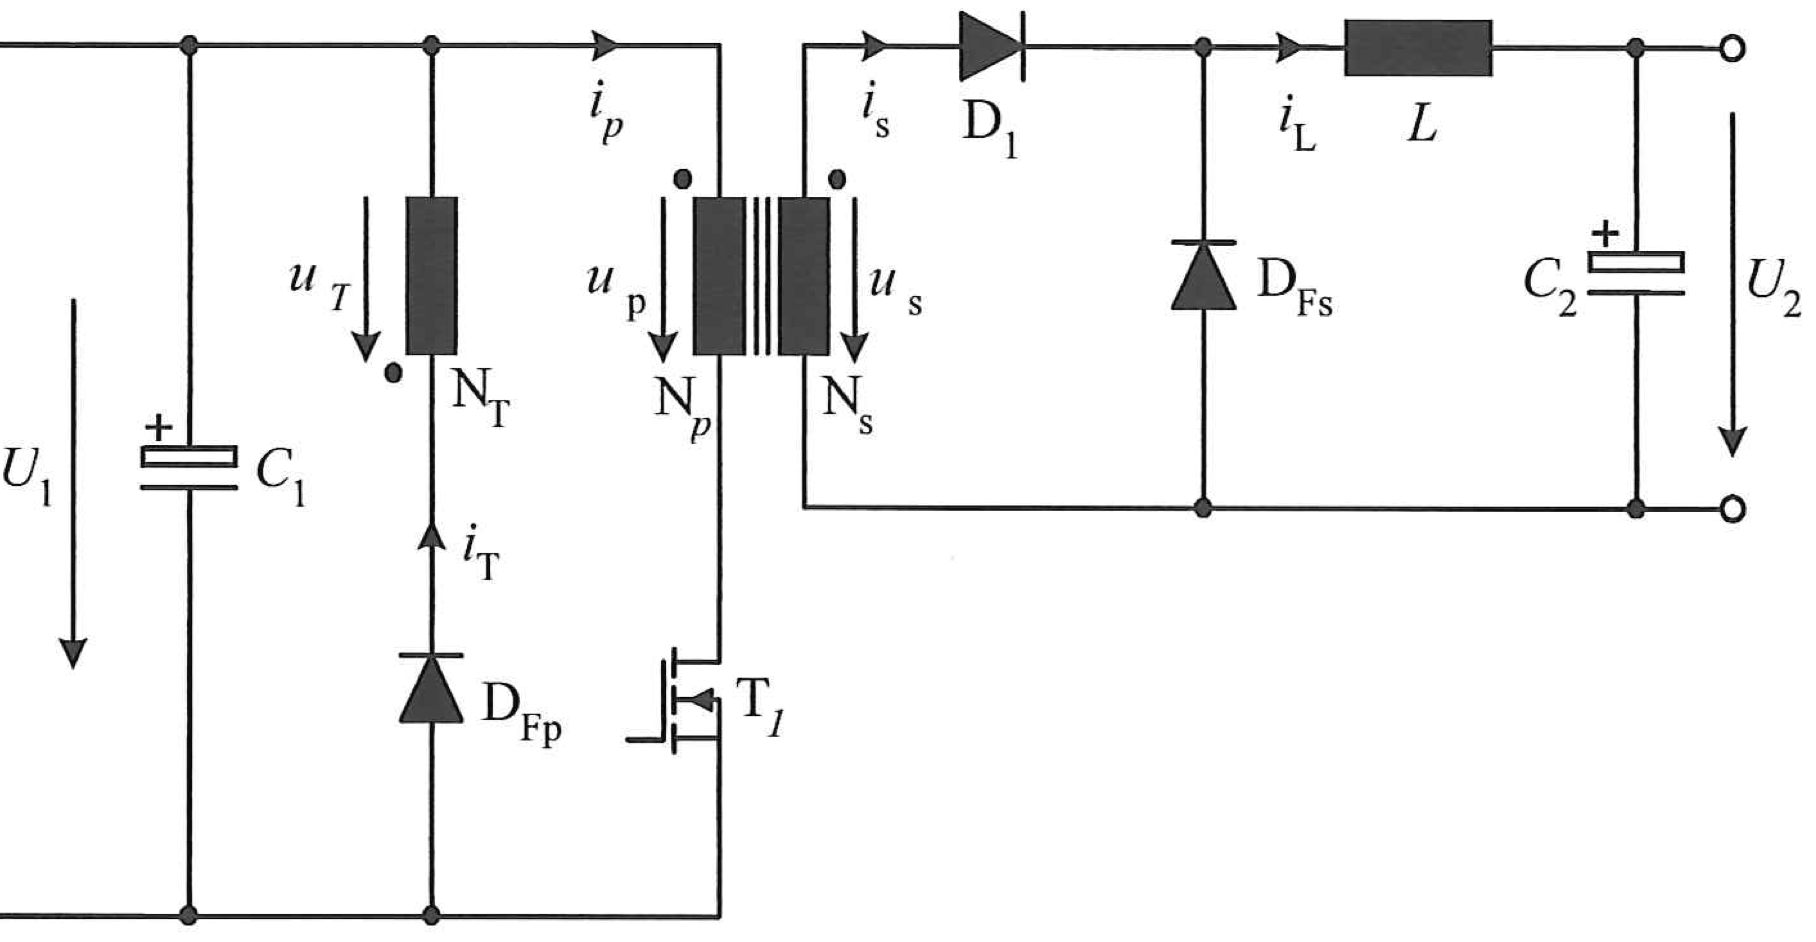
\includegraphics[width=1.0\linewidth]{img/fwd/sch.png}%
  % {\begin{align*}
  %   \hat{I}_1 &= \frac{U_1}{L_1}D_1T_p & \hat{I}_1N_1 &= \hat{I}_2N_2
  % \end{align*}}

  Der Trafo dient nur dem Energietransfer. Ideal wird keine Energie gespeichert. Der Magnetkern sollte möglichst hohe Permeabilitäte, also keinen Luftspalt, aufweisen. 
  &
  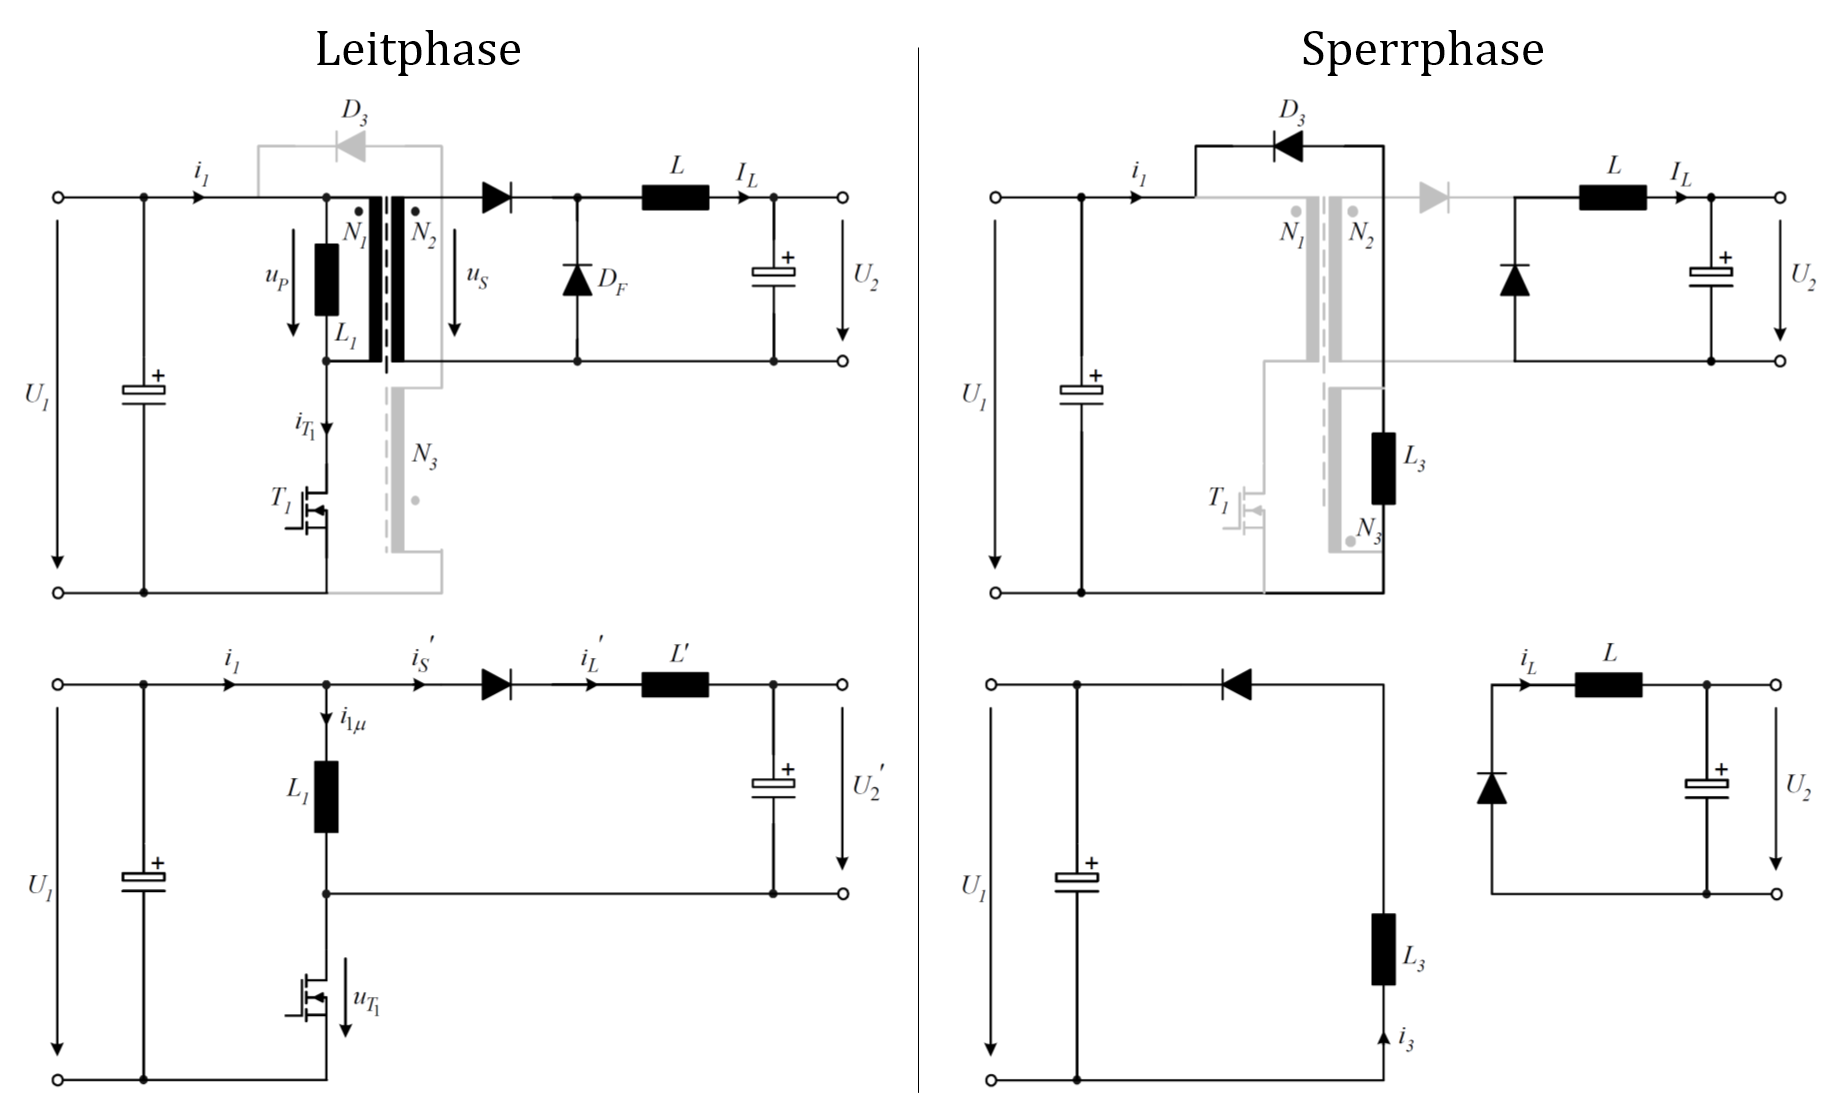
\includegraphics[width=\linewidth]{img/fwd/phasen.png}%
\end{tabular}
  
\subsection{Ideale Kopplung}
Zum Abbau der Magnetisierungsenergie wird die Entmag.Wicklung $N_3$ eingeführt. Sie führt die Mag.Energie durch einen Strom $i_3$ in $U_1$ oder an Ausgang.


\begin{tabular}{p{0.30\linewidth}|p{0.65\linewidth}}
  $0<t<t_1$ Leitphase, $T_1$, $D_2$ leitet, $D_F$ sperrt &
  {\begin{align*}
    u_p &= U_1 & 
    U_s &= \frac{N_2}{N_1}u_p = \frac{N_2}{N_1}U_1 & 
    u_{DF} &= \frac{N_2}{N_1}U_1
    \\
    i_\mu &= \frac{U_1}{L_\mu}t &
    i_1 &= i_p = i_\mu + i_s' &
    \frac{\mathrm{d}}{\mathrm{d}t}i_s' &= \frac{\mathrm{d}}{\mathrm{d}t}i_2' = \frac{U_1-u_2'}{L}
  \end{align*}} \\ \hline

  $t_1<t<t_2$ Sperrphase, $T_1$, $D_2$ sperrt, $D_F$ leitet &
  {\begin{align*}
    u_p &= -U_1 & 
    u_{DF} &= 0
    \\
    i_\mu &= \hat{I}_\mu-\frac{U_1}{L_{1,\mu}}(t-t_2) &
    i_p &= i_\mu = -i_1
  \end{align*}} \\\hline

  $t_2<t<T_p$ Entmagnetisiert &
  {\begin{align*}
    u_p &= 0 & 
    u_{DF} &= 0
    \\
    \frac{\mathrm{d}}{\mathrm{d}t}i_2' &= -\frac{u_2'}{L}
    i_p &= i_\mu = i_1 = 0
  \end{align*}}
\end{tabular}
  
  $D_{D1,max}$: In der Sperrphase liegt $U_1$ an der dritten Wicklung an, welche eine Spannung an der Sekundärwicklung verursacht.
  \begin{align*}
    U_{T1,max} &= U_1 - U_p &
    U_p &= -\frac{N_P}{N_T}U_T = -\frac{N_P}{N_T}U_1
    \Aboxed{D_1T_p\frac{U_1}{L} &= D_2T_p \frac{N_P}{N_T}\frac{U_1}{L} }
    \\
    U_{D_{Fs},max} &= \frac{N_S}{N_P}U_1 &
    D_{D1,max} &= \frac{N_S}{N_P}\frac{N_P}{N_T}U_1
  \end{align*}
  
% -----------------------------------------------------------------------
\vfill\null
\columnbreak
\section{Einphasen Gleichspannungswechselrichter}

\begin{tabular}{b{0.51\linewidth} b{0.4\linewidth}}
  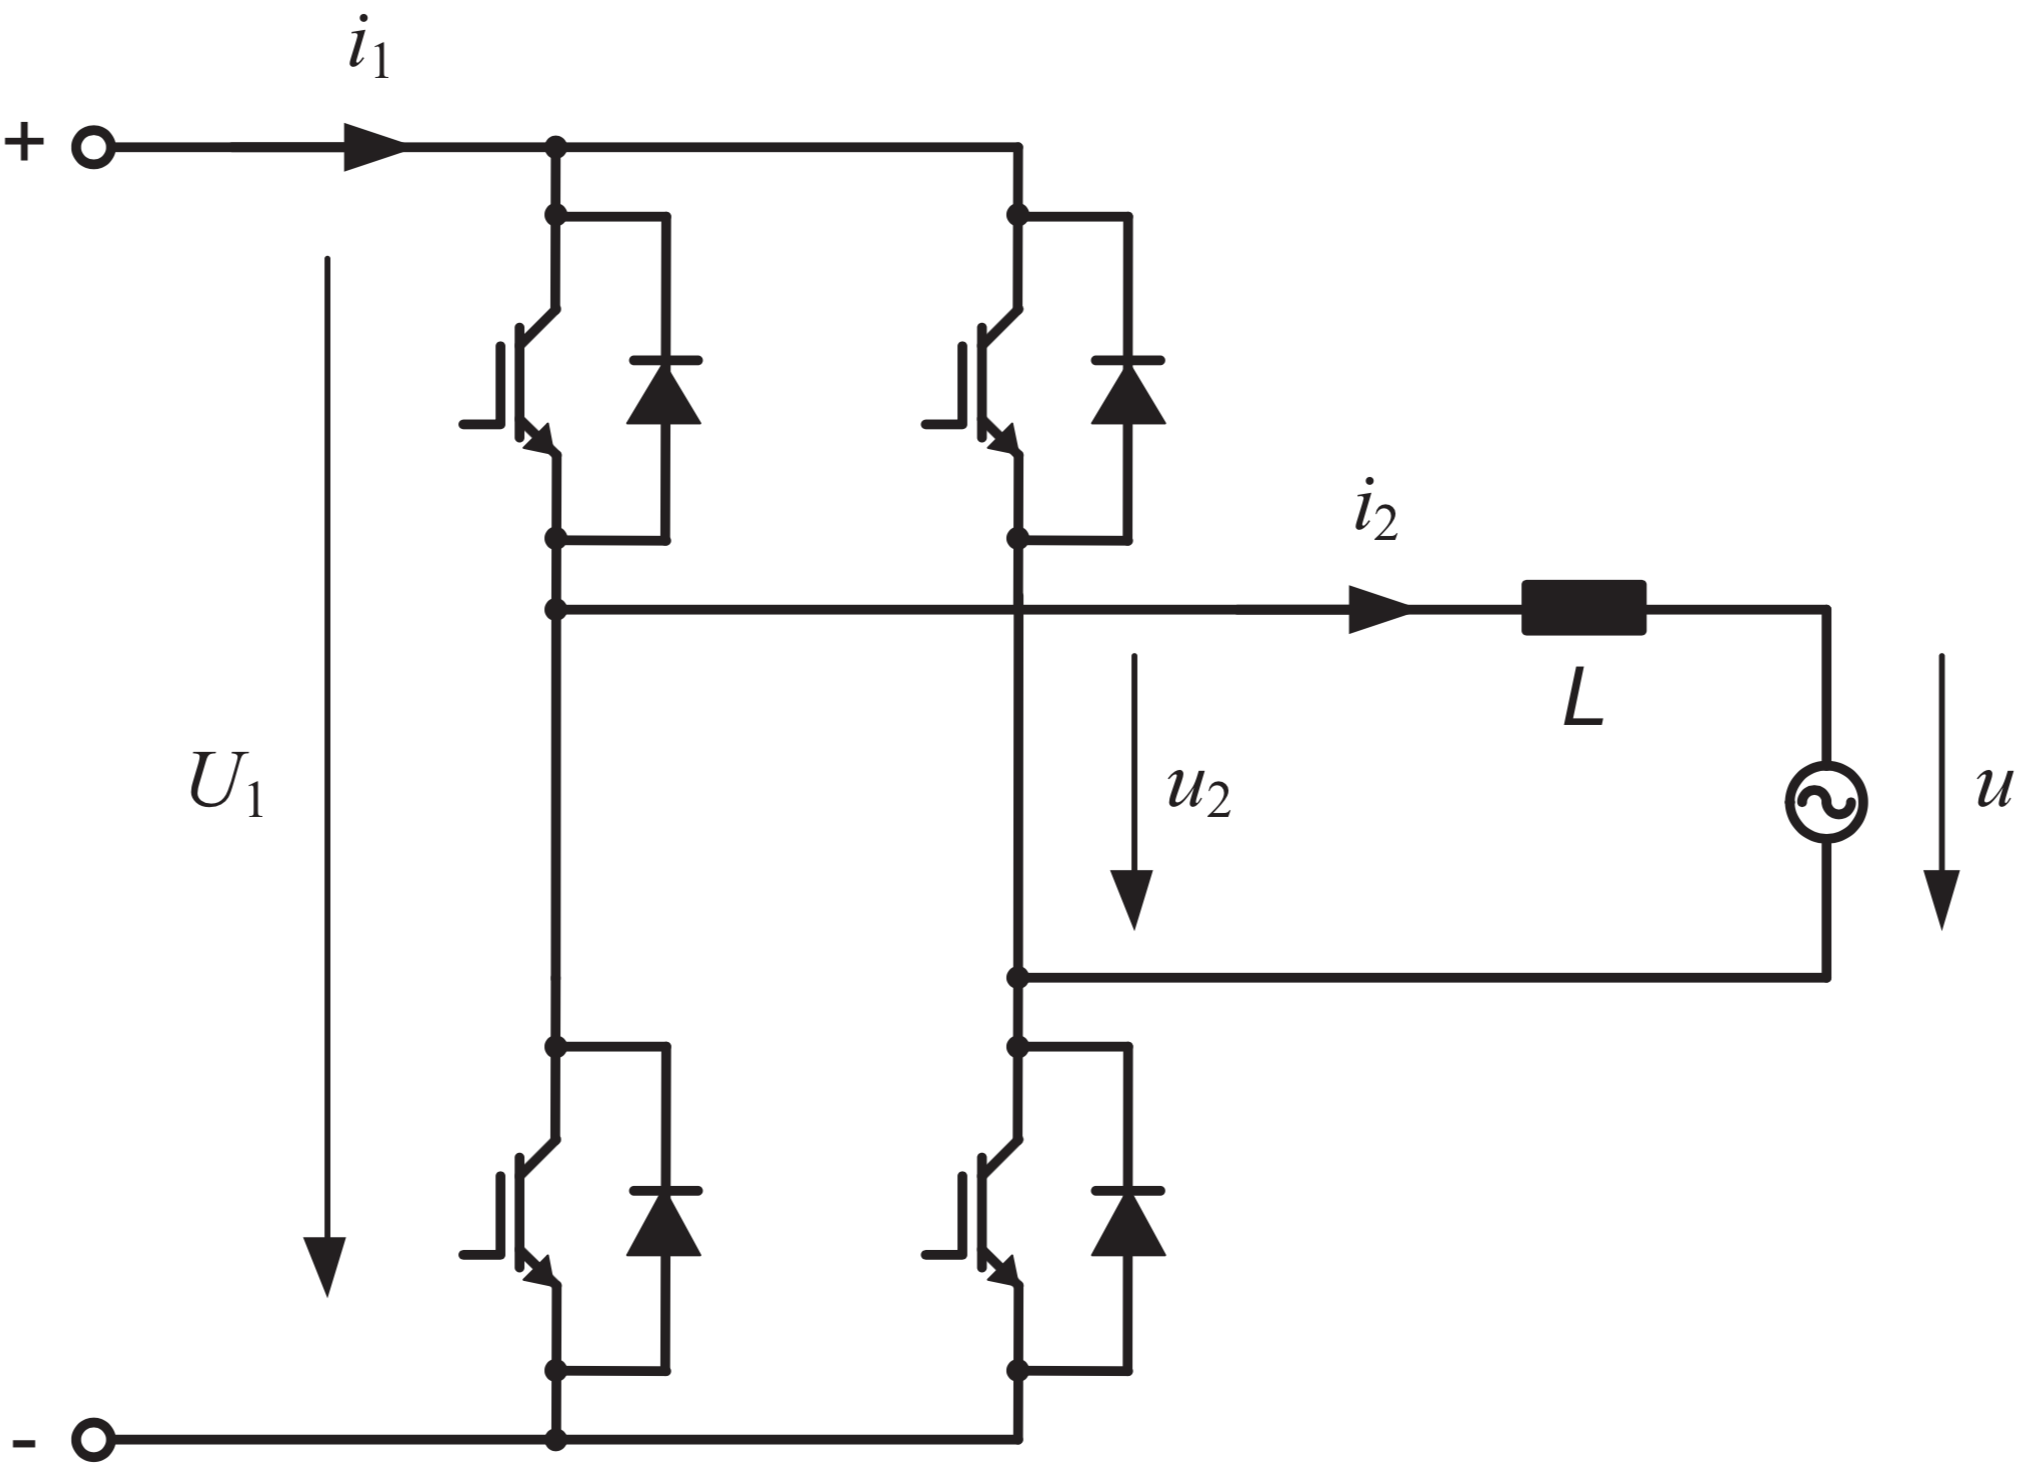
\includegraphics[width=0.8\linewidth]{img/sch_fullbridge.png}%
  % {\begin{align*}
  %   \hat{I}_1 &= \frac{U_1}{L_1}D_1T_p & \hat{I}_1N_1 &= \hat{I}_2N_2
  % \end{align*}}

  % Der Trafo dient nur dem Energietransfer. Ideal wird keine Energie gespeichert. Der Magnetkern sollte möglichst hohe Permeabilitäte, also keinen Luftspalt, aufweisen. 
  &
  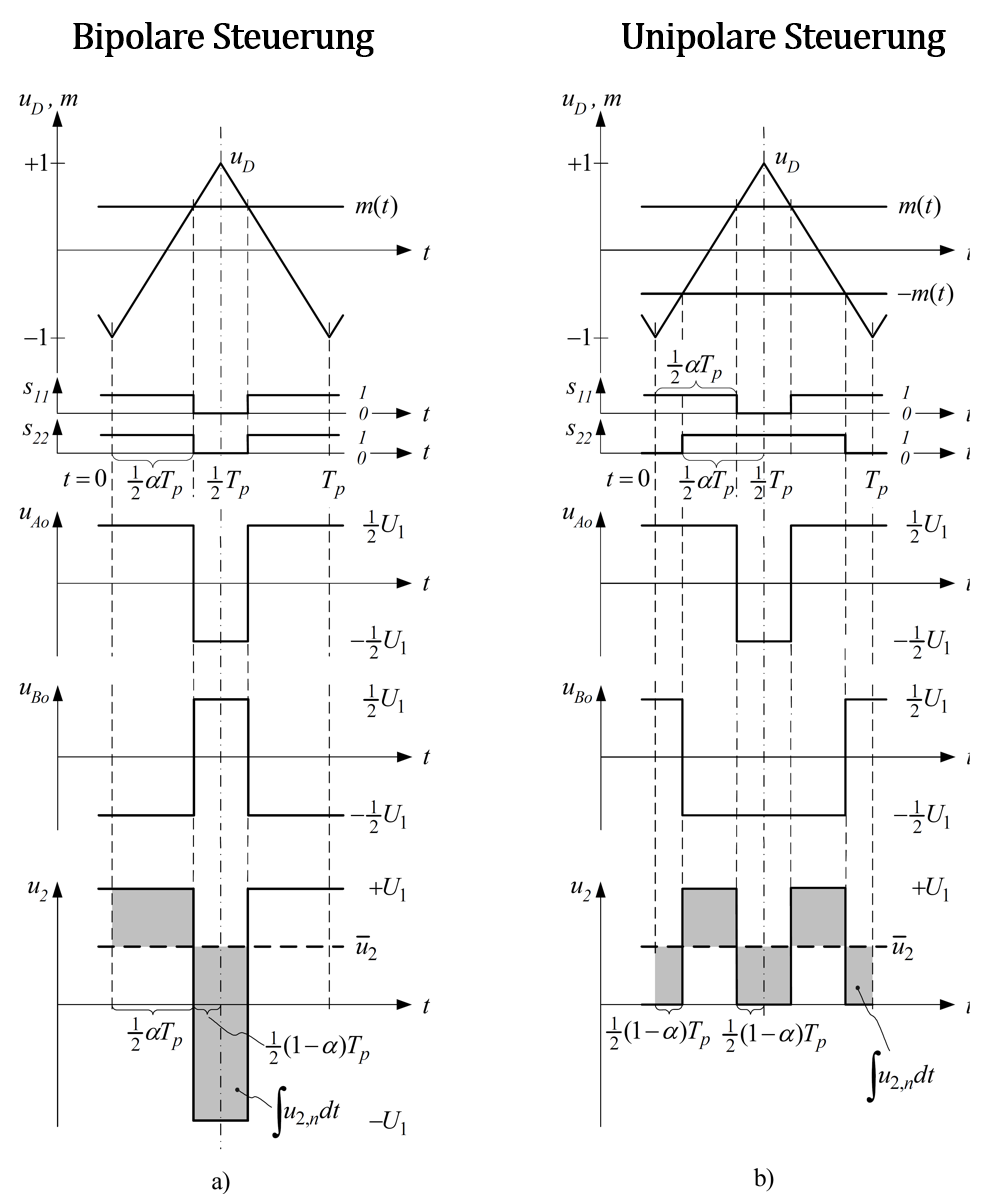
\includegraphics[width=\linewidth]{img/dcac/mod.png}%
\end{tabular}
  

\subsection{Bipolare Steuerung}
Das Steuersignal $m(t)$ wird mit einem Truagersignal $u_D$ mit Pulsperiode $T_P$ verschnitten. $\alpha(t) relative Einschaltdauer$. $m_s,\alpha_s$ für sinusförmigen Mittelwert $\bar{u}_2$. $M$ Modulationstiefe.

\begin{align*}
  u_2 &= \begin{cases} +U_1,&u_D < m(t),\\-U_1, & u_D > m(t). \end{cases} &
  \alpha(t) &= \frac{1+m(t)}{2} &
  \bar{u}_2 &= \frac{2}{T_P}\Int_{0}^{T_P/2}u_2(t)\mathrm{d}t = m(t)U_1
  \\
  m_s(t) &= \frac{\bar{u}_2}{U_1} = M\sin(\omega_2t+\delta) &
  \alpha_s(t) &= \frac{1}{2} + \frac{1}{2}M\sin(\omega_2t+\delta) &
  M &= \frac{\hat{U}_{2,(1)}}{U_1}
\end{align*}

\subsection{Unipolare Steuerung}
Es wird neben $m(t)$ eine invertierte Modulationsfunktion $-m(t)$ verwendet. Umschalten zwischen $+U_1$ und $0$ für $\bar{u}_2>0$ oder $-U_1$ und $0$ für $\bar{u}_2<0$. Die Frequenz der Ausgangsspannungsschwankund wird verdoppelt. Es gelten dieselben Beziehungen wie bei der bipolaren Steuerung.

\subsection{Vergleich}

\begin{align*}
  \textup{THD} &= \frac{U_{2,n,\textup{rms}}} {U_{2,(1),\textup{rms}}} = \frac{\sqrt{U_{2,\textup{rms}}^2-U_{2,(1),\textup{rms}}^2}}{U_{2,(1)\textup{rms}}}
\end{align*}
\begin{align*}
  &\text{Unipolar} \\
  &u_{2,\textup{rms}}^2 = U_1^2m(t) &
  U_{2,\textup{rms}}^2 &= \frac{2}{\pi}U_1M &
  U_{2,(1),\textup{rms}} &= \frac{1}{\sqrt{2}}U_1M &
  \textup{THD} &= \sqrt{\frac{4}{M\pi}-1}
  \\
  &\text{Grundfrequenztaktung} \\
  &U_{2,\textup{rms}}^2 = U_1^2 &
  U_{2,(1),\textup{rms}} &= \frac{1}{\sqrt{2}}\hat{U}_{2,(1)} = \frac{2\sqrt{2}}{\pi}U_1 &
  \textup{THD} &= \sqrt{\frac{\pi^2}{8}-1}
\end{align*}

% -----------------------------------------------------------------------

\vspace*{\fill}
% You can even have references
\rule{0.3\linewidth}{0.25pt}\\
Good Luck!
%\scriptsize
%\bibliographystyle{abstract}
%\bibliography{refFile}
\end{multicols}
\end{document}
